\documentclass[fancy, masters]{byuthesis}
% Class options are simple/fancy and masters/phd.
% Leave options blank for defaults.
% Defaults are simple for document style, and masters for degree type.


%%%%%%%%%%%%%%%%%%%%%%%%%%%%%%%
% Custom options and packages %
%%%%%%%%%%%%%%%%%%%%%%%%%%%%%%%
% Define path to figure files
\graphicspath{{figures/}}

% Define sequences of Latin text to fill space in example documents
% (not needed for your thesis -- delete or comment out if you'd like)
\usepackage{blindtext}


%%%%%%%%%%%%%%%%%%%%%%%%%%%%%%
% Define title page elements %
%%%%%%%%%%%%%%%%%%%%%%%%%%%%%%
% Thesis title for required BYU title page
\title{Forecasting Novel Modes across\\
Multiple Model Frameworks}

% On the custom title page, use the same title, but format as you like
\customtitle{Forecasting Novel Modes across\\
Multiple Model Frameworks}

% Your name goes here:
\author{Christopher Day}

% This is the date of graduation
\date{April 2021}

% If your degree is not a PhD or MS, then you can overwrite the degree using
\degree{Master of Science}

% Your department
\department{Department of Civil and Construction Engineering}

% The names of your committee members
\committeechair{Gregory S. Macfarlane}
  \committeemember{Grant G. Schultz}
  \committeemember{Gustavious P. Williams}

% Include any keywords you would like for your thesis/dissertation
\keywords{activity-based model, multi-agent simulation, novel transport modes, ActivitySim, BEAM}


%%%%%%%%%%%%%%%%%%%%%%%%%%%%%%%%%%
% ---Bibliography source file--- %
%%%%%%%%%%%%%%%%%%%%%%%%%%%%%%%%%%
	\usepackage{algorithm}
\usepackage{algpseudocode}
\usepackage{dsfont}
\usepackage{pdflscape}
\usepackage{graphicx}
\usepackage{mathtools}
\usepackage{eqparbox}
\usepackage{makecell}
	\usepackage{booktabs}
\usepackage{longtable}
\usepackage{array}
\usepackage{multirow}
\usepackage{wrapfig}
\usepackage{float}
\usepackage{colortbl}
\usepackage{pdflscape}
\usepackage{tabu}
\usepackage{threeparttable}
\usepackage{threeparttablex}
\usepackage[normalem]{ulem}
\usepackage{makecell}
\usepackage{xcolor}


%%%%%%%%%%%%%%%%%%%%%%%%%%%%%%%%%%
% ---Bibliography source file--- %
%%%%%%%%%%%%%%%%%%%%%%%%%%%%%%%%%%
%  Default is references.bib
\bibliography{}

\newlength{\cslhangindent}
\setlength{\cslhangindent}{1.5em}
\newlength{\csllabelwidth}
\setlength{\csllabelwidth}{3em}
\newlength{\cslentryspacingunit} % times entry-spacing
\setlength{\cslentryspacingunit}{\parskip}
% for Pandoc 2.8 to 2.10.1
\newenvironment{cslreferences}%
  {}%
  {\par}
% For Pandoc 2.11+
\newenvironment{CSLReferences}[2] % #1 hanging-ident, #2 entry spacing
 {% don't indent paragraphs
  \setlength{\parindent}{0pt}
  % turn on hanging indent if param 1 is 1
  \ifodd #1
  \let\oldpar\par
  \def\par{\hangindent=\cslhangindent\oldpar}
  \fi
  % set entry spacing
  \setlength{\parskip}{#2\cslentryspacingunit}
 }%
 {}
\usepackage{calc}
\newcommand{\CSLBlock}[1]{#1\hfill\break}
\newcommand{\CSLLeftMargin}[1]{\parbox[t]{\csllabelwidth}{#1}}
\newcommand{\CSLRightInline}[1]{\parbox[t]{\linewidth - \csllabelwidth}{#1}\break}
\newcommand{\CSLIndent}[1]{\hspace{\cslhangindent}#1}

\providecommand{\tightlist}{%
  \setlength{\itemsep}{0pt}\setlength{\parskip}{0pt}}

%%%%%%%%%%%%%%%%%%%%%%%%%%
% --- Begin Document --- %
%%%%%%%%%%%%%%%%%%%%%%%%%%
\begin{document}


%%%%%%%%%%%%%%%%%%%%%%%%%%%%%%%%%%%%%%%%%%%%%%%%%%%%%%%
% --- Front matter (probably don't need to change)--- %
%%%%%%%%%%%%%%%%%%%%%%%%%%%%%%%%%%%%%%%%%%%%%%%%%%%%%%%
	\frontmatter

	\titlepage
	\clearpage

	\customtitlepage
	\clearpage


    \begin{abstract}
  The advent of novel transport modes has challenged forecasters to develop new methods of capturing behavior and estimating service capabilities. Bike share, e-scooter, ride hail, and autonomous vehicles have been forecasted with activity-based models, multi-agent simulations, spatial analysis, survey data and statistical methods, and even machine learning approaches. Methodologies to model new transport technologies are dissimilar and difficult to access. In this paper, we examine novel mode forecasts generated by different activity-based model and multi-agent simulation mode choice combinations. Using ActivitySim as the activity-based model and BEAM as the multi-agent simulation, we establish 10 different mode choice combinations to analyze ride hail service capabilities for a Salt Lake City, Utah case study region. By analyzing ride hail ridership, utilization, and wait times we determine two effective approaches to modeling novel modes using a linked activity-based model and multi-agent simulation. We also determine that linking an activity-based model and a multi-agent simulation is a valid methodology to forecasting novel modes, especially if novel mode choice is kept to only one of those modeling tools. Lastly, we conclude that using the combination of path, person, and location type variables to calculate the mode choice utility is more effective than only using path type variables. Overall, the results of our research give direction to those struggling to forecast new transport technologies with the current disarray of modeling approaches.
  \end{abstract}
  	\clearpage


    \begin{acknowledgments}
  I would first like to acknowledge my advisor and friend, Dr.~Gregory Macfarlane, for teaching me everything I know. Without you, this thesis and my future career would be boring and stupid. I found a work to love and enjoy while researching under your supervision, and for that I will forever be grateful. I express gratitude as well to Dr.~Shultz and Dr.~Williams for being on my advisory committe and helping me finish my thesis. I would also like to acknowledge the United States Department of Transportation (USDOT) for funding my research. Thank you to the members of the T-SCORE center, especially Dr.~Gregory Erhardt, Jawad, and Vedant for their friendship and help with tackling BEAM. A special shoutout to Nate Lant and Hayden Atchley for working on ActivitySim and BEAM even when we had no idea what we were doing. Together, we got this thing done. I am enormously grateful as well to Zachary Needell at Lawrence Berkeley National Laboratory for working with the T-SCORE team and I in our efforts to tame BEAM. Wihtout you, none of this would have been possible. An additional thanks to Wasatch Front Regional Council, especially Chad, Josh, and Bert for sharing data and working with our group. I express sincere gratitude for my family members and their patience and support as I conducted this research. Especially, thank you to my wife Megan, because without her I would probably be dead. She convinced me to apply for this research position, held down the fort at home, let me work every Saturday for 3 years, and was patient with me everytime I went insane staring at my computer screeen. I appretiate you all. Finally, thank you to the BYU tennis courts and Kevin Lunt, because you guys helped me stay sane day after day.

  Students should acknowledge funding sources. They may also use the
  acknowledgment page to express appreciation for the committee members, friends
  or family who provided assistance in research, writing or technical aspects of
  the dissertation, thesis or selected project. Acknowledgements should be simple
  and in good taste.
  \end{acknowledgments}
  	\clearpage

	\tableofcontents*
	\clearpage

	\listoffigures
	\clearpage

	\listoftables
	\clearpage

	\nomenclature{$c$}{Speed of light in a vacuum inertial frame}
\nomenclature{$h$}{Planck constant}
\nomenclature{$\mathit{Re}$}{Reynolds number}
\nomenclature{$\mathbf{x}$}{State vector}
\nomenclature{$\alpha$}{Angle of attack}
\nomenclature{$\beta$}{Sideslip angle}
\nomenclature{$\gamma$}{Climb angle}
\nomenclature{$p$}{Roll rate}
\nomenclature{$q$}{Pitch rate}
\nomenclature{$r$}{Yaw rate}
\nomenclature{$P$}{Covariance matrix}

\printnomenclature
	\clearpage

%%%%%%%%%%%%%%%%%%%%%
% --- Main Body --- %
%%%%%%%%%%%%%%%%%%%%%
	\mainmatter

\hypertarget{introduction}{%
\chapter{Introduction}\label{introduction}}

\hypertarget{problem-statement}{%
\section{Problem Statement}\label{problem-statement}}

The advent of novel transport modes has challenged forecasters to develop new methods of capturing behavior and estimating service capabilities. The usage of bike share, an affordable and sustainable bike rent program, has been modeled countless times each with a different methodology (e.g., Hyland et al. (2018), Biehl et al. (2019), Cho \& Shin (2022), W. Li \& Kamargianni (2018), Welch et al. (2020), X. Zhou et al. (2019), Song et al. (2019)). Forecasters are riddled with determining the best technique for understanding who uses e-scooters (public electric scooters) and in what locations they would be most effective (e.g, Zuniga-Garcia et al. (2022), Tuli et al. (2021), W. Zhang et al. (2021), M. Lee et al. (2021), H. Lee et al. (2021), Hosseinzadeh et al. (2021)). In general, forecasters have modeled micromobility (bike share, e-scooters, e-bikes) in many ways, yet few have attempted to model multiple novel modes simultaneously (e.g., Reck et al. (2021), Campbell et al. (2016), Lazarus et al. (2020), McKenzie (2019), Younes et al. (2020)). Ride hail and ride share, which allow users to hire a driver, behave differently than regular car modes. Given their unique nature, understanding their behavior and service capabilities is particularly challenging (e.g., Kang et al. (2021), Y. Li et al. (2020), Dong (2020), Dean \& Kockelman (2021)). Forecasters have even attempted to understand the effects of autonomous vehicles, even though to date little to no data exists on fully-autonomous vehicles (e.g., Mo et al. (2022), Wadud \& Chintakayala (2021), F. Zhou et al. (2020)). New transport technologies are becoming more prominent each day, and equally so is the need to accurately capture their behavior.

Various efforts have been made to model novel transport modes accurately, but since methodologies are dissimilar with one another it remains difficult to determine the best approach. For example, some forecasters have chosen to model novel transport modes with an activity-based model, which uses daily activity patterns as the central tool to model an individual's travel behavior (e.g., Xu et al. (2019), Muhammad et al. (2019), Macfarlane et al. (2021)). Other forecasters use multi-agent simulation, which focuses on modeling the interactions between different agents, to understand new transport technologies (e.g., Shimizu et al. (2013), Sánchez et al. (2019), Hörl, Ruch, et al. (2019)). In general, many forecasters have modeled novel modes in activity-based models, multi-agent simulations, or other modeling frameworks by using a logit based regression analysis, which uses a function to understand characteristics of the modes (e.g., Welch et al. (2020), M. Lee et al. (2021), Dong (2020)). Some chose a simpler approach, spatial analysis and geography data, to understand new transport technologies (e.g., Hyland et al. (2018), Cho \& Shin (2022), Hosseinzadeh et al. (2021)). Forecasters have even attempted to use machine learning to better understand novel modes! (e.g., X. Zhou et al. (2019)). With limited data on novel transport modes, the validity of the results from each approach can be difficult to verify.

\hypertarget{purpose-of-research}{%
\section{Purpose of Research}\label{purpose-of-research}}

In this paper we examine novel mode forecasts generated by different activity-based model and multi-agent simulation mode choice combinations. By examining the ride hail service capabilities between each combination, we hope to understand which mode choice combination is best, or if a best combination even exists. Since only limited data on novel mode usage exists, it seems logical to test different mode choice combinations to determine the best way to model new transport technologies. Overall, this paper aims to give forecasters additional direction in how to model novel transport modes.

\hypertarget{lit}{%
\chapter{Literature Review}\label{lit}}

As discussed in the introduction, forecasters model novel transport modes using activity-based models, multi-agent simulation, spatial analysis, machine learning, and more. Since our research mainly focuses on activity-based models, multi-agent simulation, and the link between them both, understanding the other model frameworks is not within the scope of this project. For this reason, the following literature review outlines the strengths and weaknesses of activity-based models and multi-agent simulation, the previous attempts to model novel transport modes with activity-based models and multi-agent simulation, and the brief literature of those who have attempted to reconcile two modeling approaches within the same study. Within the scope of this paper however, it is not practical to provide a comprehensive review of all activity-based models, multi-agent simulations, or paired modeling approaches.

\hypertarget{lit-abm}{%
\section{Introduction to Activity-based Models}\label{lit-abm}}

Activity-based models are transportation models that construct daily activity patterns from behavioral choice models. They predict what activities are conducted, where those activities are conducted, the length and time of those activities, and the people involved in those activities. This detailed approach to modeling behavior allows forecasters to understand travel at a high level both spatially and temporally. According to Philip et al. (2013), activity-based models generate travel demand by first modeling activity demand. Understanding the idea that all travel is generated by activities is essential to accurately representing the way people travel. This link between activity and travel allows activity-based models to model behavior especially well, which is particularly advantageous when modeling novel modes. Bowman (1998) also explains that activity-based models have choice models that use utility theory and logit based regression to estimate behavior. These choice models accept an array of inputs relating to person, household, and regional data, to better capture the travel behavior of any particular region.

In addition to representing behavior accurately, another advantage to using activity-based models is that there is modal consistency between trips on the same tour (e.g., Nayak \& Pandit (2022), Hasnine \& Nurul Habib (2021), Knapen et al. (2021), Gomes et al. (2021)). Nayak \& Pandit (2022) explains that other existing models fail to consider the ``interrelationships among trips'' performed by the same individual on the same tour. For example, if you were to take your car to the gym, and then stop by the store on the way back home, wouldn't you also use your car to get from the store back to your home? Individuals will act similarly among trips of the same tour, and activity-based models account for this natural tendency. Hasnine \& Nurul Habib (2021) explains that tour based modeling is the core of activity-based models; ``tackling'' every trip within a tour is essential to understanding the dynamics that exists between trips. Gomes et al. (2021) explains that trip-based models, unlike activity-based models, disregard trip sequences, trips made by the same individual, and the relationship between trips and activities. Chaining trips of the same individual together, within the same tour, helps ensure modal consistency within models.

Knowing the advantages that activity-based models provide when modeling travel behavior, many forecasters use activity-based models to model the behavior and service capabilities of novel modes. For example, some new technologies that have been modeled with activity-based models are car-sharing (e.g., Nguyen et al. (2022), Q. Li et al. (2018)) and autonomous vehicles (e.g., Xu et al. (2019), Vyas et al. (2019)). Nguyen et al. (2022) modeled one-way car-sharing services with an activity-based model because the modal consistency between trips allowed them to track vehicle demand, pricing, and other parameters. Xu et al. (2019) modeled privately-owned autonomous vehicles with an activity-based model as a way to better understand their impact on household travel patterns, including very large households. Macfarlane et al. (2021) used an activity-based model to model on-demand wheelchair accessible microtransit vehicles. This activity-based model generated daily activity patterns for all individuals in the region, including those who were wheelchair dependent. With those plans they were able to simulate microtransit vehicles with a microsimulation tool, and process the results to understand service capabilities. Tzouras et al. (2022) conducted a quantitative study of activity-based models for modeling e-scooters. They agreed that activity-based models are an effective vehicle to describe the spatiotemporal variation in e-scooters, and novel modes in general. Muhammad et al. (2019) used an activity-based model to model bike share and the concept of Mobility as a Service, which aims to make public transport a pay-per-service or monthly subscription. Many forecasters elect to use activity-based models to model new transport technologies because of the behavioral representation and modal consistency they provide.

Although there are advantages to using activity-based models to model novel modes, forecasters must consider the various weaknesses that exist when using activity-based models. One of the biggest shortfalls within most activity-based models is that travel times are averaged along travel links (e.g., RSG (2016), Mahmoudi et al. (2021)). For example, although Nguyen et al. (2022) used an activity-based models to model one-way car sharing, they noted that it used the BPR function to estimate travel time. The BPR function is a regression function that estimates average travel time based on arrival flows. When using the BPR function to estimate smaller time intervals though, it becomes inconsistent. For this reason, Nguyen et al. (2022) noted that it was more difficult to verify the service capabilities of the car-sharing modes. Similarly, on-demand microtransit vehicles should be modeled with variable wait time; the difference between a 4 minute wait and a 17 minute wait is significant when traveling. Macfarlane et al. (2021) recognized this shortcoming, and elected to estimate the on-demand travel time by using a multi-agent simulation on top of an activity-based model. Overall, since travel time is a significant part of the mode choice utility, average travel time is a shortfall when modeling novel modes.

Another typical weakness present in most activity-based models is their focus on individual-based behavior, instead of household-based behavior. Although it is widely known that many decisions made by humans are done collectively, little effort has been made to model travel based on intra-household interactions and group decisions making (J. Zhang \& Fujiwara, 2006). However, some forecasters have attempted to account for this shortfall (e.g., J. Zhang \& Fujiwara (2006), Neutens et al. (2008), Soo (Kum Lin (2009)). Neutens et al. (2008) and Soo (Kum Lin (2009) in particular attempted to extend individual-level travel to household-level travel by assigning certain tasks (activities) to different household individuals, verifying that schedules within the same households were coherent. J. Zhang \& Fujiwara (2006) developed a household utility function to help represent the ``diverse intra-household interactions''. Travel behavior is more than just a set of strung together activities, and certain interactions (e.g., household-based decisions) are important to consider when modeling transport modes.

\hypertarget{lit-mas}{%
\section{Introduction to Multi-agent Simulation}\label{lit-mas}}

An alternative to activity-based models for forecasting novel modes is multi-agent simulation. Multi-agent simulation, usually synonymous with the term microsimulation, models interactions between individual agents. Multi-agent simulation is a desirable tool because it allows analysis to be done on both the individual and group levels; individualized decisions can be explored (e.g., Kamel et al. (2019)) as well as agent to agent interactions (e.g., Bazghandi (2012), Amblard et al. (2015), Siebers \& Aickelin (2008)). These agent to agent interactions and individualized decisions allow forecasters to better understand why a novel mode may or may not be chosen. For example, multi-agent simulation allows forecasters to know exactly how many users participate in a novel transport mode, which type of users are interested in a novel transport mode, and if other agents played a role in the novel transport mode choice decision.

Along with modeling unique agents, another reason multi-agent simulation is advantageous for modeling novel modes is its transportation network and capacity constraint. Transportation networks are visual representations of the actual road networks, and allow forecasters to see the transportation decisions made by each agent. In addition to being visual tools, agents are coded to the network allowing them to interact with attributes of the network itself. For example, Dia (2002) used a real traffic network in their model to simulate areas of high traffic congestion. Within the model, agents could notice high congestion areas and some of them would chose to take an alternate route. Due to the interaction between individual agents and roadway conditions, realistic travel behavior is captured on a global scale. Djavadian \& Chow (2017) and Fujii et al. (2017) also used a real transportation network to capture realistic global travel behavior. Djavadian \& Chow (2017) explored the usage of flexible mobility systems like taxi and carpool and Fujii et al. (2017) explored mixed traffic consisting of cars, pedestrians, and trams. Fujii et al. (2017) even enhanced the basic transportation network system by coding various virtual driving lanes at each intersection, thus making the network even more realistic. Cetin et al. (2002) describes two more benefits of road networks: one, vehicles are subject to remain on network links for a certain amount of time (according to their travel speed) and, two, a storage capacity exists for each link that once met, no more vehicles can enter. By using a transportation network, the travel times, speeds and congestion become reliable model outputs, and therefore, the travel times, speeds, and congestion of novel modes are easily modeled. Multi-agent simulation uses unique agents with a realistic transportation network to create attainable and reliable model outputs.

Due to the advantages that multi-agent simulation provides, various forecasters have elected to use them to model novel transport modes. For example, Kamel et al. (2019) chose to use a multi-agent simulation to model shared autonomous vehicles because decision-making was done on an individual level. This granularity helped the researchers understand how user preferences affected the modal split of shared autonomous vehicles. Hörl, Ruch, et al. (2019) also analyzed shared autonomous vehicles with a multi-agent simulation, mainly to take advantages of the detailed network dynamics. By utilizing the detailed network, the researchers were able to estimate the system performance, wait times, and cost of various autonomous vehicle fleets. Other analyses have been completed on other novel modes like with shared mobility (e.g., Ciari et al. (2016), Shimizu et al. (2013), Becker et al. (2020)) and electric vehicles (e.g., Sánchez et al. (2019)). Specifically, Ciari et al. (2016) summarizes a multitude of research done to understand demand for car-sharing with the multi-agent simulation model MATSim. In this research, they note that although multi-agent simulation provides an extensive level of detail, it does not necessarily equate to real world accuracy. A model rich in detail and with extensive behavioral rules, however, allows innovative transportation technologies to be analyzed efficiently in a world where ``solid behavioral knowledge does not yet exist''. Therefore, by using MATSim, Ciari et al. (2016) surpassed the typical pitfalls of modeling a new transport mode like car-sharing, and adequately modeled the individual travel decisions with a high temporal and spatial resolution. Similarly, Becker et al. (2020) used MATSim to model different shared mobility services (car-sharing, bike-sharing, ride-hailing). By using a multi-agent simulation, multiple novel transport modes could be analyzed simultaneously within the same model. Many forecasters continue to analyze new transportation technologies with multi-agent simulation because its inherit advantages are helpful to understanding service capabilities.

Although the advantages within multi-agent simulation are useful to modeling novel modes, forecasters must be aware of the weaknesses within these models as well. For example, although Kamel et al. (2019) used multi-agent simulation to model shared autonomous vehicles, they understood that the homogeneous behavior structure may decrease the accuracy of their results. A homogeneous behavior structure means that all agents within the model have similar preferences when facing decisions, like mode choice. This renders results to be less accurate since oftentimes people choose a specific mode based solely on their personal preference. Tchappi et al. (2018) reviews many of the advantages of a holonic multi-agent simulation (holonic meaning to divide the system into dependent groupings), but acknowledges the weakness that driver behavior is not homogeneous. The other major weakness of multi-agent simulations is their high computational requirements (e.g., Siebers \& Aickelin (2008), Cetin et al. (2002), Adler et al. (2005)). In order to adequately model the individualized nature of every agent, while mapping each agent to a detailed road network, affluent computing power is needed. The need for a high processing computer and sufficient computing time is indeed a limitation for some forecasters.

Another inherit weakness of most multi-simulation models is its focus on trips-based modeling. Most multi-simulation models only simulate agents on a trip level, ignoring the tour-based framework present in most activity-based models. Figure \ref{fig:fig-mode-compare} provides a visual example of this difference. If a person wants to go to their work activity by train, an activity-based model knows that they can either walk or take transit to their gym activity. Contrastingly, a multi-agent simulation bases mode choice on the first trip of the day. This means that a multi-agent simulation will determine the optimal mode to go to the gym in, and then figure our how to get to work based on the first trip mode. In addition, an activity-based model knows that when a person leaves for lunch from their work activity, they will be returning back to their work activity after lunch. This means that the person is able to leave their car at work and possibly walk or take transit to and from their lunch activity. In a multi-agent simulation though, if someone goes to lunch, they will most likely take their car as to not abandon their vehicle for the rest of their day. It is clear that a multi-agent simulation's mode choice is less representative of how people actually transport themselves during the day. An activity-based model provides a better representation of mode choice. In this research we attempt to link a activity-based model and a multi-agent simulation tool as to use the advantages of both models to better model novel transport modes.

\begin{figure}

{\centering 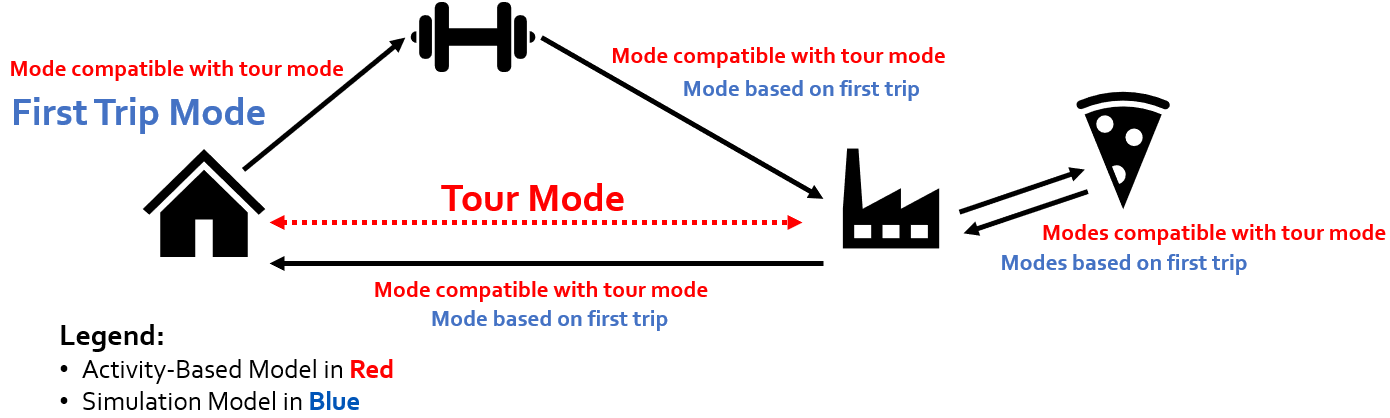
\includegraphics[width=1\linewidth]{pics/abm-mas-compare} 

}

\caption{Mode choice in activity-based models and multi-agent simulation.}\label{fig:fig-mode-compare}
\end{figure}

\hypertarget{limited-attempts-to-pair-two-disparate-modeling-approaches}{%
\section{Limited Attempts to Pair Two Disparate Modeling Approaches}\label{limited-attempts-to-pair-two-disparate-modeling-approaches}}

The varying strengths and weaknesses within both activity-based models and multi-agent simulation point to possibly using both approaches to understand novel mode behavior. Yet few forecasters have attempted to reconcile or pair these two disparate approaches in order to better understand novel mode behavior. However, one example of reconciling the traditional approaches is with the system MITO (e.g., Moeckel et al. (2020), Zwick et al. (2021)). MITO stands for Microsimulation Transport Orchestrator, and its primary purpose is to overcome the limitations of the traditional trip-based model while being easier to implement than the traditional activity-based model. Like a multi-agent simulation, MITO simulates each agent individually, however, MITO also restricts agents of the same household with a travel time budget. This travel time budget influences destination choice, and ensures that agents participate in sensible activities (e.i. those household members who commute to work are less likely to perform shopping and discretionary activities). MITO includes a simplified activity schedule builder, allows forecasters to add attributes, allows agent tracing, and is not as computationally heavy as traditional multi-agent simulations (Moeckel et al., 2020). Zwick et al. (2021) used MITO to estimate travel demand and MATSim, a multi-agent simulation tool, to simulate that demand. By pairing together MITO and MATSim, the researchers were able to gather service criteria for a novel transport mode: pooled on-demand ride hailing vehicles.

Traditionally, MATSim implements a feedback loop to determine mode choice instead of using a discrete choice model. For example, if in one iteration too many agents choose a car mode and travel times go up, in the next iteration some agents will opt to use an alternative mode. This process continues until equilibrium is found between the supply and demand. Some researches have attempted, however, to pair together a discrete mode choice model with MATSim in attempt to shorten the number of iterations needed to be run. For example, Hörl, Balać, et al. (2019) discovered that by using a discrete choice model within MATSim, no irrelevant mode choice decisions were made. This indeed, lead to less iterations being run. However, although initial modal decisions were more accurate than the default MATSim model, the discrete choice model added a layer of complexity. Accurate and consistent data is needed in order for the discrete choice model to work effectively. This need for more data gives the model runners less freedom. Hörl, Balać, et al. (2019) mentions that their research was merely an introduction to the concept, and further research is desirable to understanding all the benefits of linking discrete choice and simulation based tools.

Another example of pairing together two different modeling approaches is with an activity-based model and a dynamic traffic assignment model (e.g., L. Zhang et al. (2018), Pendyala et al. (2017), Shiftan (2000)). Dynamic traffic assignment models are useful as they understand time-dependent interactions, simulate individual agents, capture congestion, and can model new transportation technologies (L. Zhang et al., 2018). Pairing together activity-based models and dynamic traffic assignment models is of great interest to forecasters, as their structures are similar and together they produce results at a finer level of detail. L. Zhang et al. (2018) paired together InSITE, an activity-based model, with DTALite, a dynamic traffic assignment model, to model travel demand in the Baltimore-Washington region. Their conclusion was that the integrated model performed better than the singular InSITE activity-based model. Overall, they determined that the integrated model produced better results, but was more challenging to run and required consistent upkeep to ensure consistency between models.

To the authors knowledge, no previous literature exists on pairing together an activity-based model with a multi-agent simulation for the purpose of modeling novel mode behavior. (We view the work done by Lant (2021) as an exception, because this research was specifically designed to build on top of that work). Yet both activity-based models and multi-agent simulation have their own unique strengths when it comes to modeling novel modes. Could using both an activity-based model and a multi-agent simulation within the same study maximize each model's strengths while limiting each model's weaknesses? There exists a need to understand which methodology is best for modeling novel modes, or if a best methodology even exists. The objective of this study is to better understand the effects of using different mode choice combinations between varying activity-based models and multi-agent simulation combinations. We aim to use these results to provide forecasters guidance as to which choice model combination they should use to model novel modes.

\hypertarget{methods}{%
\chapter{Methods}\label{methods}}

We developed a series of experiments to understand the relative importance of activity-based and multi-agent simulation in forecasting the uptake of novel modes. These experiments were performed using ActivitySim as the activity-based model and BEAM as the multi-agent simulation. We used the Salt Lake City, Utah region as a case study for our experiments. Since ride hailing vehicles were an emerging technology in the region at the time of our study, we deemed it the appropriate novel transport mode to model in our experiments. The following section outlines the methodology for which we were able to model a novel transport mode with differing activity-based model and multi-agent simulation mode choice combinations.

\hypertarget{meth-asim}{%
\section{ActivitySim as the Activity-based Model}\label{meth-asim}}

ActivitySim is an activity-based simulator used to generate plans for millions of agents each with their own demographic attributes (Gali et al., 2008). Instead of independently modeling each trip, ActivitySim simulates each individual by calculating their daily travel diaries and schedules. Long term decisions are made first, and then shorter term decisions are calculated based on those long term decisions ({``ActivitySim,''} 2021). Overall, ActivitySim is an advanced activity-based model with the same advantages and disadvantages described in Section \ref{lit-abm}.

\hypertarget{novel-modes-in-activitysim}{%
\subsection{Novel Modes in ActivitySim}\label{novel-modes-in-activitysim}}

ActivitySim was chosen as the activity-based model in this research because built into its framework are the novel modes of ride hail and pooled ride hail. Specifically, ride hail and pooled ride hail fall under one of the four nested tiers of ActivitySim's nested logit model. This means that ride hail is a unique modal option not characterized by being an auto, non-motorized, or transit type mode. Figure \ref{fig:fig-asim-nest} displays the four tiers of the nested logit along with the modal alternatives of each tier (MTC, 2012). These modal alternatives represent the alternatives available in both ActivitySim's tour based and trip based mode choice model. When determining the mode to use on a trip, ActivitySim first calculates the tour mode and subsequently calculates the trip mode based on the tour mode selection (See Figure \ref{fig:fig-mode-compare}). Person attributes, path attributes, location attributes, tour purpose value, and more all play a role in calculating the mode choice decision.

\begin{figure}

{\centering 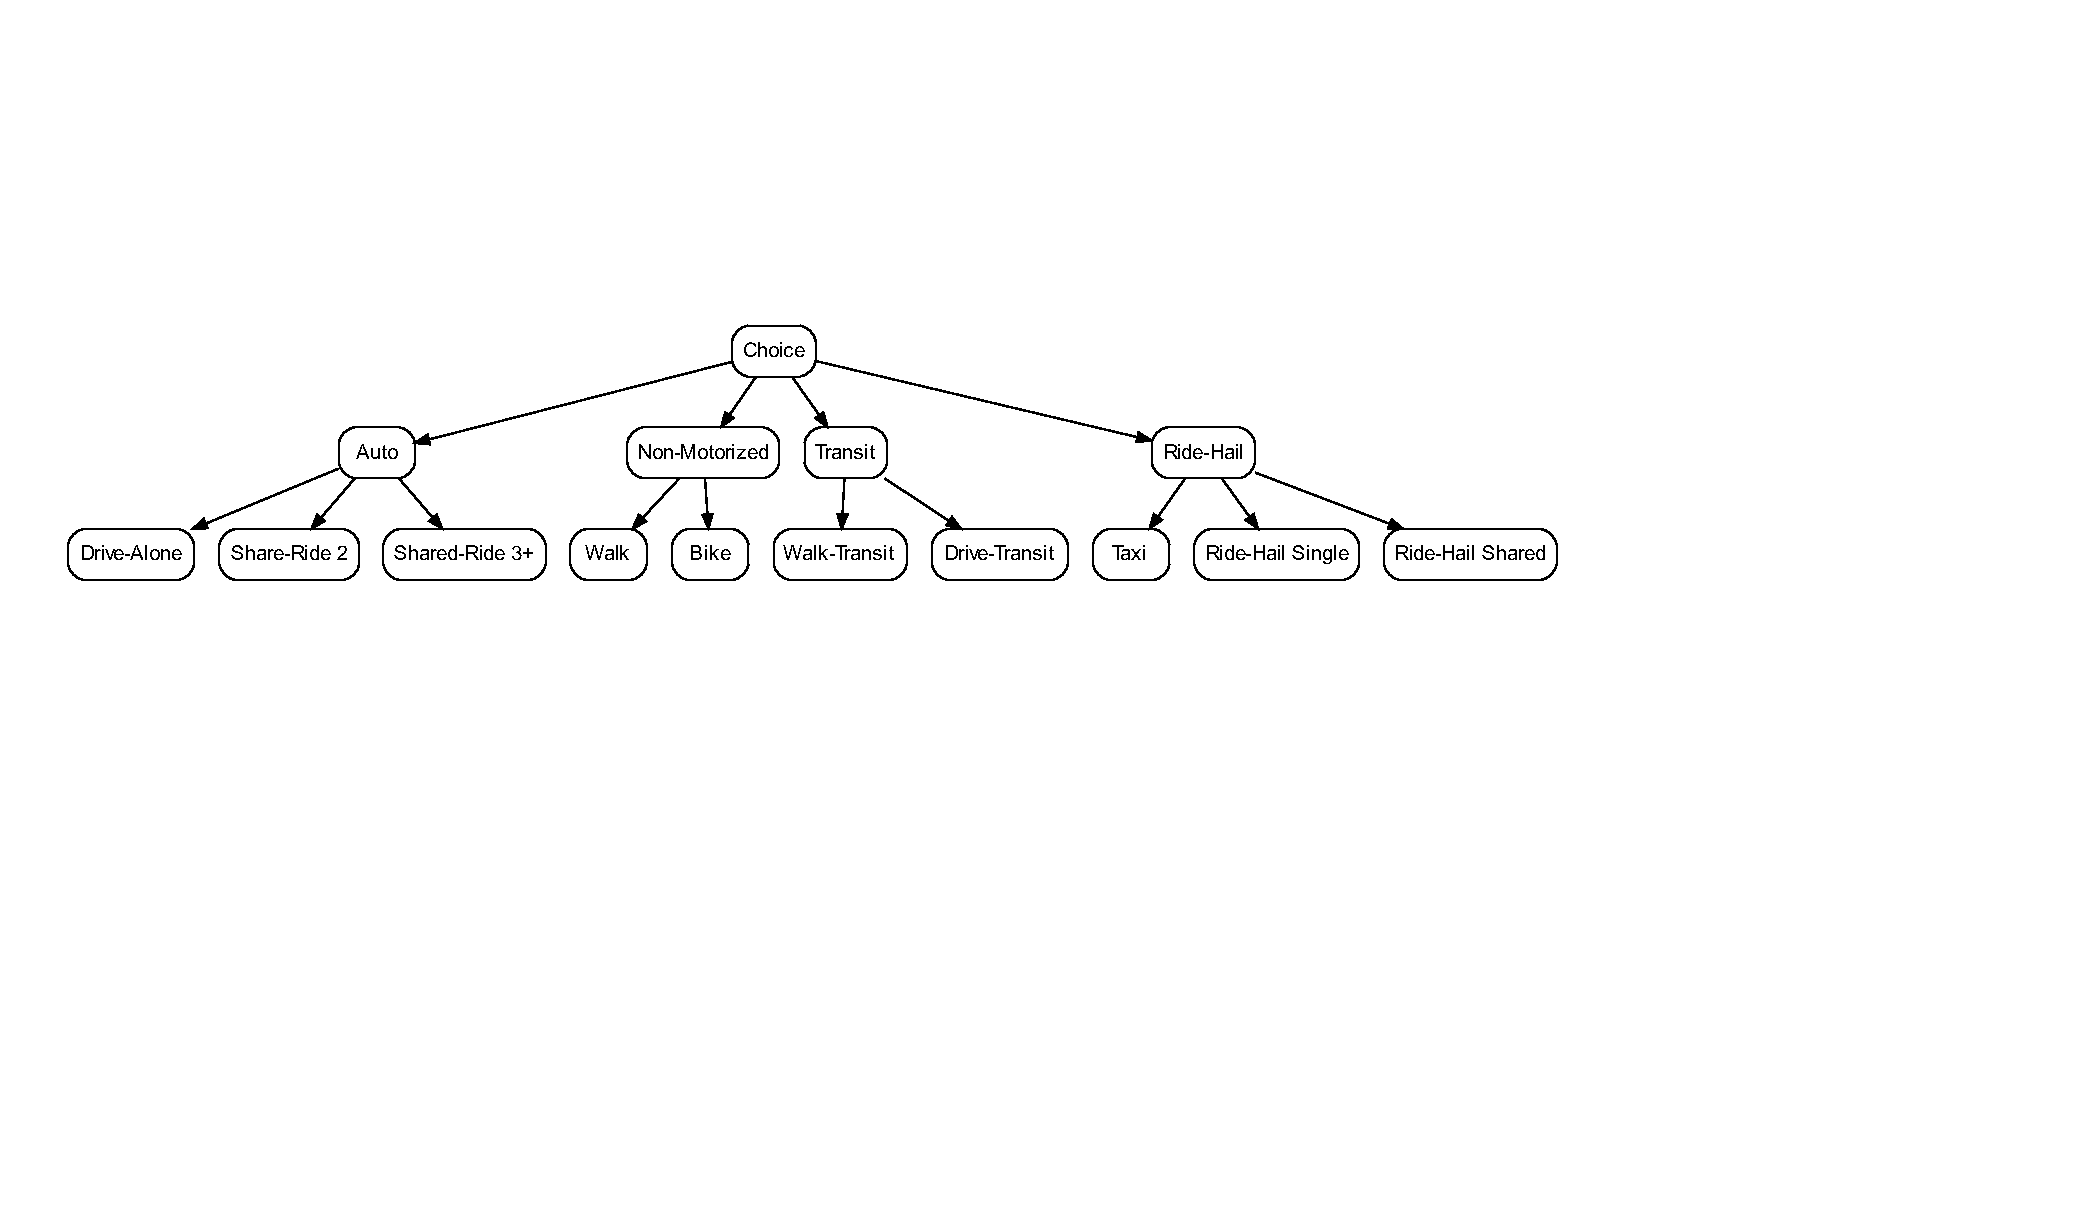
\includegraphics[width=.7\textwidth,trim = {5cm 6.5cm 12.5cm 4cm}]{thesis_files/figure-latex/fig-asim-nest-1} 

}

\caption{The nested logit model used in ActivitySim.}\label{fig:fig-asim-nest}
\end{figure}

In addition to using specific attributes to determine the mode choice decision, ActivitySim also sets default parameters for choosing ride hail and pooled ride hail vehicles. For example, a base fare, cost per mile, cost per minute, and cost minimum are all set before model runs. These values can be changed between model runs, but are held constant for all ride hail vehicles in the same model run. In addition, a mean wait time is used to help calculate the total travel time of ride hail vehicles. This means that all mode choice decisions to choose ride hail vehicles use the same wait time in the utility calculation. There is no variability in wait time between one agent using ride hail against another. One exception however, is that there are 5 different mean wait time values depending on the location of the ride hail request. Mean wait times also differ between single ride hail trips and shared ride hail trips. There is also one parameter for the maximum allowed wait time for a ride hail vehicle. Overall, it was essential to use ActivitySim to model ride hail vehicles because the mode choice structure fostered accurate behavioral representation and modal consistency between trips. However, ActivitySim's absence in using variable wait time to calculate the ride hail choice utility led us to also modeling ride hail vehicles with a multi-agent simulation (See Section \ref{meth-beam}).

\hypertarget{activitysim-configured-to-the-case-study-region}{%
\subsection{ActivitySim Configured to the Case Study Region}\label{activitysim-configured-to-the-case-study-region}}

ActivitySim was configured to the case study region by first gathering and generating the input data. Three input files were necessary in order to run ActivitySim:

\begin{enumerate}
\def\labelenumi{\arabic{enumi}.}
\tightlist
\item
  A synthetic population of the agents within the study area.
\item
  A zonal socioeconomic data file describing the characteristics of each zone.
\item
  A set of skims that describe the cost and travel times of all modes between all zones.
\end{enumerate}

A synthetic population is a generated population with specific individual attributes that add up to the regional characteristics as a whole. We generated the synthetic population using a software called PopulationSim (PopulationSim, 2021). We used a ``seed'' table, which represented information of a subset of the population, and a set of ``targets'', which represented demographic data of smaller areas of the region, to run PopulationSim (Lant, 2021). The zonal socioeconomic data file stores zonal characteristics regarding household, worker, and other activity type information. This file was created using data from Wasatch Front Regional Council (WFRC) (WFRC, 2019), Utah Automated Geographic Reference Center (AGRC, 2021), and the synthetic population when necessary. The skims are large matrices showing travel times and costs between every set of zones within the area of study. Included in these skims were further details regarding differences in modes, distances, wait times, etc. (Lant, 2021). We used pre-generated skims from WFRC (2019), with some slight adjustments, in our run of the ActivitySim model.

After generating the necessary input files, we calibrated and validated the ActivitySim model to better represent decisions made in the Salt Lake region. The process of calibrating and validating the ActivitySim model to the Salt Lake region was conducted by Lant (2021). The purpose of the calibration and validation was to ensure that the outputs generated by ActivitySim matched target regional values. Specifically, trip productions, trip distributions, and mode choices were tested to match the given target values from the four-step model from WFRC (2019). The details behind the exact calibration and validation process are discussed by Lant (2021), and therefore will not be described in detail within this paper. However, we did conduct one additional calibration measure beyond that which Lant (2021) completed. Due to some slight adjustments made after the initial calibration of ActivitySim, we elected to re-calibrate ActivitySim's tour mode choice parameters. Using the 2012 household travel survey as our targets, we improved ActivitySim to model a more accurate total modal distribution of the region (WFRC, 2019). The fully calibrated and validated ActivitySim model was then ready to run and generate activity plans for the case study region.

\hypertarget{meth-beam}{%
\section{BEAM as the Multi-agent Simulation Tool}\label{meth-beam}}

BEAM stands for Behavior, Energy, Autonomy, and Mobility and is a multi-agent simulation tool being developed by Lawrence Berkeley National Laboratory and UC Berkeley Institute for Transportation Studies (BEAM, 2022). As an extension of MATSim, it simulates individual agents using both within day replanning and across-day replanning to maximize individual utility. Overall, BEAM shares many of the same advantages and disadvantages of most multi-agent simulations as described in Section \ref{lit-mas}.

\hypertarget{novel-beam}{%
\subsection{Novel Modes in BEAM}\label{novel-beam}}

BEAM was chosen as the multi-agent simulation in this research because of its integration with transportation network companies (TNCs), or ride hail and pooled ride hail vehicles. (BEAM also supports plug-in electric vehicle modeling, however, this feature was not used within our research.) Along with the TNC type mode options, BEAM supports many of the regular choices as well, such as car, walk, bike, walk-to-transit, and drive-to-transit. Default BEAM uses a simple multinomial logit choice model for determining which mode any particular agent will use on any particular trip. Only a few variables are used to calculate the modal alternative: cost, travel time, number of transfers, and an alternative specific constant (ASC) (BEAM, 2022).

BEAM was also chosen as the multi-agent simulation in this research because of how it implements ride hailing vehicles. BEAM uses a greedy asynchronous ride hail matching algorithm that also supports pooled trips. The algorithm works by first, requiring agents to send a request for a ride hail vehicle, and then by second, matching the closest vehicle to that agent. For the algorithm to work, BEAM requires the modeler to input a ride hail vehicle fleet. This fleet is a simple file that describes the number of ride hailing vehicles available in the region, their starting locations, their working hours, their seating capacity, and other specifications. BEAM assigns these vehicles to the roadway network, where they ``roam'' the streets awaiting requests. The ride hail algorithm permits a more realistic ride hail modeling structure. For example, agents make a request to take a ride hail vehicle, expect a variable wait time dependent on their geographic location, and may not even be able to take the vehicle if there is no availability! All these attributes are similar to how using ride hail is in real life, and represent the true advantages to modeling ride hail with BEAM.

\hypertarget{meth-beam-link}{%
\subsection{Linking the Mode Choice of ActivitySim and BEAM}\label{meth-beam-link}}

In order to use BEAM in conjunction with ActivitySim, however, its mode choice model was updated to be more consistent with ActivitySim's mode choice model. More specifically, three changes were made to the choice structure:

\begin{enumerate}
\def\labelenumi{\arabic{enumi}.}
\tightlist
\item
  Adding a Tour Purpose Attribute
\item
  Adding Person, Path, and Location Attributes to the Utility Equation
\item
  Adding New Modal Alternatives
\end{enumerate}

First, a tour purpose attribute was added at the trip level, to be used when making trip-based modal decisions. ActivitySim's default utility parameters are segmented by tour purpose, auto ownership, and mode; therefore, adding a tour purpose level attribute was essential to calculating the mode choice utility similar to ActivitySim.

Second, multiple person, path, and location related attributes were added to use in the mode choice utility equations. The MTC example of Activityim (the example referenced in this research) uses 25 different variables in the utility calculation (MTC, 2012). So, BEAM was adjusted to use values like wait time, transit proximity, distance, age, household size, and more on top of the default variables to calculate modal utility. This was done by gathering path and location variables from the BEAM router and person level variables from the input files. ASCs were copied directly from the MTC ActivitySim example, and then calibrated later on. Overall, one input file was created which housed all path, person, and location type parameters on a tour purpose, auto ownership, and modal level.

The last major adjustment made to the BEAM software was adding new modal alternatives. The most important difference between the ActivitySim modal options and the BEAM modal options is the inclusion of carpooling vehicles (HOV2 and HOV3). HOV2 means High Occupancy Vehicle with 1 passenger (2 people in the vehicle) and HOV3 means High Occupancy Vehicle with 2 or more passengers (at least 3 people in the vehicle). The BEAM software was adjusted to include HOV2 and HOV3 type modes, including a distinction between drivers and passengers of those vehicles. Within the code, HOV2 and HOV3 modes were provided as modal options by transforming an existing car option into an HOV option. This allowed car travel statistics to be transferred over to the carpooling modes, which were essential to calculating the utility.

BEAM's default mode choice model was adjusted dramatically to be more closely aligned with how the MTC example of ActivitySim handles mode choice (MTC, 2012). As a way to better understand the complexity of the new mode choice model in BEAM, two pseudocode algorithms are provided. Specifically, the algorithms are meant to provide clarification on how BEAM's new mode choice model works.

Algorithm 1 describes the process behind determining the mode choice alternatives for each agent. This process occurs for every agent for every trip. Two procedures are presented within the first algorithm. The first procedure is called DetermineHOVAlternatives. This procedure was added to the BEAM code as a way to include carpooling options. In this procedure the HOV alternatives are created from already existing options created by the R5 router (Conveyal, 2022). (The R5 routing engine helps BEAM accomplish multi-modal routing). Basically if a car, HOV2, or HOV3 mode is already created from the router, then both HOV2 and HOV3 options are provided. If car is not provided by the router, then passenger HOV options are provided. Passenger HOV modes, called HOV\_TELEPORT, are completed by teleporting agents from origin to destination. The second procedure within Algorithm 1 describes the process behind determining the final modal alternatives. It essential states that if the current mode is already chosen, then that mode remains as the only alternative to choose from. However, if no mode is currently chosen for the trip, the router, ride hailing, and HOV alternatives are combined and presented as the final alternatives to choose from.

\begin{algorithm} [tph]
\caption{Algorithm for Determining Mode Choice Alternatives in BEAM}
\begin{algorithmic}[1]
\Require
\State $i : origin$
\State $j : destination$
\State $n: agent$
\State $N: population$
\State $t : trip $
\State $P : plan$
\State $\vec{R}(i,j) : Router\: alternatives$
\State $\vec{RH}(i,j) : Ridehail\:alternatives$
\State $\vec{H}(i,j) : HOV\:alternatives$
\State $\vec{M}(i,j) : Final\:modal\:alternatives$
\State $C : Current\:Mode$
\State $I : Trip\:Index$
\vspace{4pt}\hrule\vspace{5pt}

\State $\vec{R} \equiv \vec{R}(i,j)$
\State $\vec{RH} \equiv \vec{RH}(i,j)$
\State $\vec{H} \equiv \vec{H}(i,j)$
\State $\vec{M} \equiv \vec{M}(i,j)$
\For {$n \in N$}
\For {$t \in P$}

\Procedure {DetermineHOVAlternatives}{$\vec{R}$, $C$}
\If {$C=None$}
  \If {$\vec{R} \ni CAR$}
    \State $\vec{H} \gets (HOV2,HOV3)$
  \ElsIf {$\vec{R} \ni HOV2$}
    \State $\vec{H} \gets (HOV3)$
  \ElsIf {$\vec{R} \ni HOV3$}
    \State $\vec{H} \gets (HOV2)$
  \ElsIf {$\vec{R} \ni WALK$}
    \State $\vec{H} \gets (HOV2\_TELEPORT, HOV3\_TELEPORT)$
  \EndIf
\Else
  \State $\vec{H} \gets None$
\EndIf
\EndProcedure
\Statex
\algstore{myalg}
\end{algorithmic}
\end{algorithm}

\addtocounter{algorithm}{-1}
\begin{algorithm}
\caption{continued}
\begin{algorithmic} [1]
\algrestore{myalg}
\Procedure {DetermineFinalModalAlternatives}{$\vec{R}$, $\vec{RH}$, $\vec{H}$, $C$, $I$}
\If {$C = DRIVE\_TRANSIT \lor BIKE\_TRANSIT$}
  \If {$I = 0$}
    \If {$C = DRIVE\_TRANSIT$}
      \State $\vec{M} \gets (DRIVE\_TRANSIT)$
    \Else
      \State $\vec{M} \gets (BIKE\_TRANSIT)$
    \EndIf  
  \Else
    \State $\vec{M} \gets (WALK\_TRANSIT, RIDEHAIL\_TRANSIT)$
  \EndIf
\ElsIf {$C = WALK\_TRANSIT \lor RIDEHAIL\_TRANSIT$}  
  \If {$C = WALK\_TRANSIT$}
    \State $\vec{M} \gets (WALK\_TRANSIT)$
  \Else
    \State $\vec{M} \gets (RIDEHAIL\_TRANSIT)$
  \EndIf
\ElsIf {$C = HOV2\_TELEPORT \lor HOV3\_TELEPORT$}  
  \If {$C = HOV2\_TELEPORT$}
    \State $\vec{M} \gets (HOV2\_TELEPORT)$
  \Else
    \State $\vec{M} \gets (HOV3\_TELEPORT)$
  \EndIf
\ElsIf {$C = CAR$}
  \State $\vec{M} \gets (CAR)$
\Else
  \State $\vec{M} \gets \vec{R} + \vec{RH} + \vec{H}$  
\EndIf  
\EndProcedure
\EndFor
\EndFor
\Statex
\end{algorithmic}
\end{algorithm}

Algorithm 2 describes the process within BEAM for how one modal alternative is selected among all the mode choice options. Algorithm 2 is basically the pseudocode behind the process that occurs with the mulitnomial logit function. Then, after using the multinomial logit formula, the probabilities that were calculated are sampled and one final mode choice alternative is selected!

\begin{algorithm}
\caption{Algorithm for Selecting Final Modal Alternative in BEAM}
\begin{algorithmic}[1]
\Require
\State $i : origin$
\State $j : destination$
\State $n: agent$
\State $N: population$
\State $t : trip $
\State $P : plan$
\State $\vec{A}: attributes\:of\:agent$
\State $a: attribute\:value$
\State $\vec{M}(i,j) : Modal\:alternatives$
\State $m : alternative \in M(i,j)$
\State $\vec{U}(\vec{M}(i,j),\vec{A}):Utilities\:for\:alternatives$
\State $u: utility \in \vec{U}(\vec{M}(i,j),\vec{A})$
\State $\vec{c}: attribute\:coefficients$
\State $\mathds{P}: probability$
\State $Mode: chosen\:mode\:for\:agent\:(n)\:on\:trip\:(t)$
\State $f(\vec{X}):$
This function takes a vector of modes and  their probabilities of being chosen. With those probabilities it builds them into a cumulative distribution function, generates a random number and then drops the mode with the closest probability. This process continues until only one mode is left.
\vspace{4pt}\hrule\vspace{5pt}

\State $\vec{M} \equiv \vec{M}(i,j)$
\State $\vec{U} \equiv \vec{U}(\vec{M},\vec{A})$
\For {$n \in N$}
\For {$t \in P$}\Procedure {DetermineFinalModalAlternative}{$\vec{M}$, $\vec{A}$, $\vec{c}$}
\For {$m \in \vec{M}$}
  \State $u \gets \sum_{a\in \vec{A}} a \times c_a$
  \State $\vec{U} += [m,u]$
\EndFor
\State $S \gets \sum_{u\in \vec{U}}e^u$
\For {$u \in \vec{U}$}
    \State $\mathds{P}(u)\gets e^u / S$
    \State $\vec{B} +=[m, \mathds{P}(u)]$
\EndFor 

\State $Mode \gets f(\vec{B})$

\EndProcedure

\EndFor
\EndFor
\Statex
\end{algorithmic}
\end{algorithm}

\hypertarget{beam-configured-to-the-case-study-region}{%
\subsection{BEAM Configured to the Case Study Region}\label{beam-configured-to-the-case-study-region}}

BEAM was configured to the case study region by gathering the inputs, validating the utility parameter values, and calibrating the utility ASC values to the region. Gathering the BEAM input files were easy simply because the outputs generated by the calibrated ActivitySim model were used as the inputs to BEAM. Only a slight formatting change was made to these inputs; and since they were generated by the calibrated ActivitySim model, they were already configured to the Salt Lake region.

The utility parameter values used in BEAM's new mode choice model were copied directly from MTC's implementation of ActivitySim (MTC, 2012). MTC's implementation of ActivitySim was designed for the San Francisco, California region. Logically, travel behaviors such as travel time, travel distance, and number of transfers should affect people in different regions in similar ways. However, as a way to validate the use of ActivitySim's path utility coefficients in the Salt Lake region, these values are compared to values from the Utah Statewide model, the WFRC travel demand model, and the NCHRP Report 716. The Utah Statewide model is useful as it provides a rough idea of the influence of path variables in Utah as a whole (UDOT, 2021). The WFRC model model is a useful comparison as it predicts travel behavior for the same region of study used in this research project (WFRC, 2019) . NCHRP Report 716 provides a rough idea of what parameter values should look like for a generalized modeling point of view (Cambridge Systematics et al., 2012). Overall, comparing these three sets of path parameter values with the MTC ActivitySim parameter values used in BEAM helps ensure that the the utility parameters are valid.

Figure \ref{fig:hbw} shows the comparison of the path utility parameter values between all four models for home-based work trips. For the egress time, in vehicle travel time (IVTT), the number of transfers, transfer time, and the wait times, MTC's ActivitySim seems to use a very similar coefficient value as the other three models. The largest discrepancy exists with short and long walking distances. ActivitySim seems to use a value almost ten fold that of the other models. This occurs because the WFRC and Utah Statewide models cap walking distance whereas ActivitySim instead gives a high penalty for long walking distances. With this clarification, it is clear to see that ActivitySim's path coefficient values do not require calibration and were left as is.

\begin{figure}

{\centering 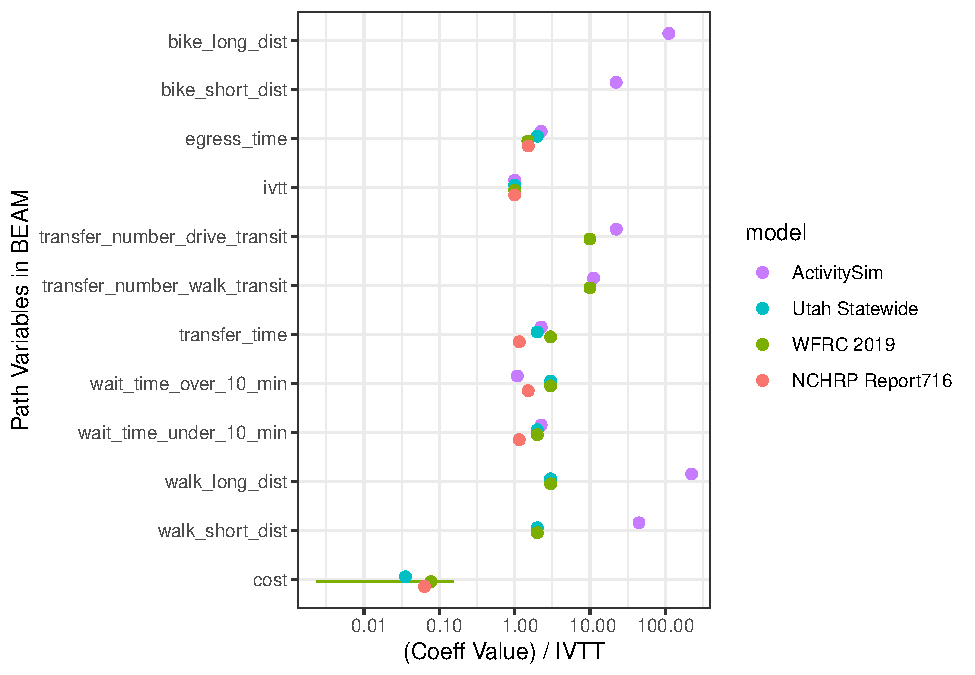
\includegraphics{thesis_files/figure-latex/hbw-1} 

}

\caption{Home-based work mode choice path coefficients model comparison.}\label{fig:hbw}
\end{figure}

Figure \ref{fig:hbs} shows the comparison of the path utility parameter values between all four models for home-based school trips. Similar to the home-based work analysis, for the egress time, IVTT, transfer time, and the wait times, ActivitySim seems to use a very similar coefficient value as the other three models. Again, the largest discrepancy exists with short and long walking distances. Since this is simply a difference between how walk distance is modeled, the discrepancy is ignored. In addition, the other three models did not have information on number of transfers. As a result, there is no comparison done with number of transfers. ActivitySim's path coefficient values do not require calibration for the home-based school parameters.

\begin{figure}

{\centering 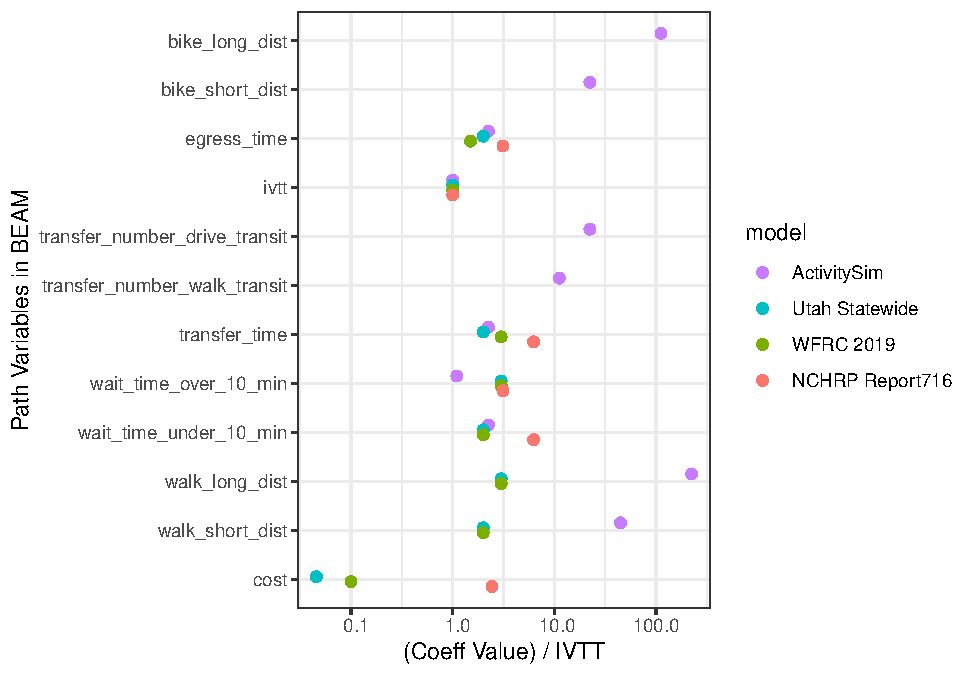
\includegraphics{thesis_files/figure-latex/hbs-1} 

}

\caption{Home-based school mode choice path coefficients model comparison.}\label{fig:hbs}
\end{figure}

Lastly, Figure \ref{fig:hbo} shows the comparison of path utility parameter values between all four models for home-based other trips. Again, besides for walk distance all variables seem to be similar between all four models. An interesting point is that for models other than ActivitySim, the cost coefficient varies greatly. Fortunately, ActivitySim bases the cost coefficient on each individual's value of time so this is not a concern. Overall, for all purpose types the coefficients used by ActivitySim are similar enough to other models that exist, and therefore do not require calibration.

\begin{figure}

{\centering 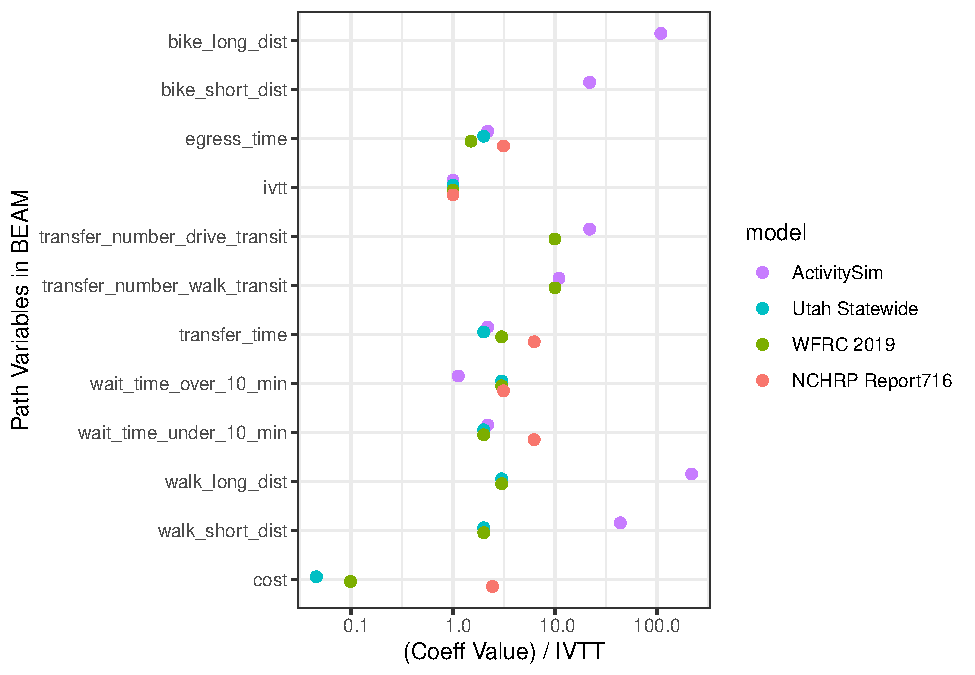
\includegraphics{thesis_files/figure-latex/hbo-1} 

}

\caption{Home-based other mode choice path coefficients model comparison.}\label{fig:hbo}
\end{figure}

After validation was completed, the last step in order to run BEAM with the case study region was to calibrate the ASC values of the mode choice model. BEAM calibration was completed by iteratively updating the ASC values using Equation \eqref{eq:eqcalib}. The number of trips totaled by tour purpose, auto ownership, and modal alternative were compared between the BEAM results and the ActivitySim results and used to adjust each ASC value. After 15 iterations of Equation \eqref{eq:eqcalib} were completed on the ASC values, the BEAM trip values were within a reasonable range to the ActivitySim target shares. Figure \ref{fig:fig-beam-calib} shows the progress of the calibration targets with the final shares after each iteration.

\begin{equation}
  NewASC = OldASC + ln(\frac{Trips_{ASIM}}{Trips_{BEAM}}) \label{eq:eqcalib}
\end{equation}

\begin{figure}

{\centering 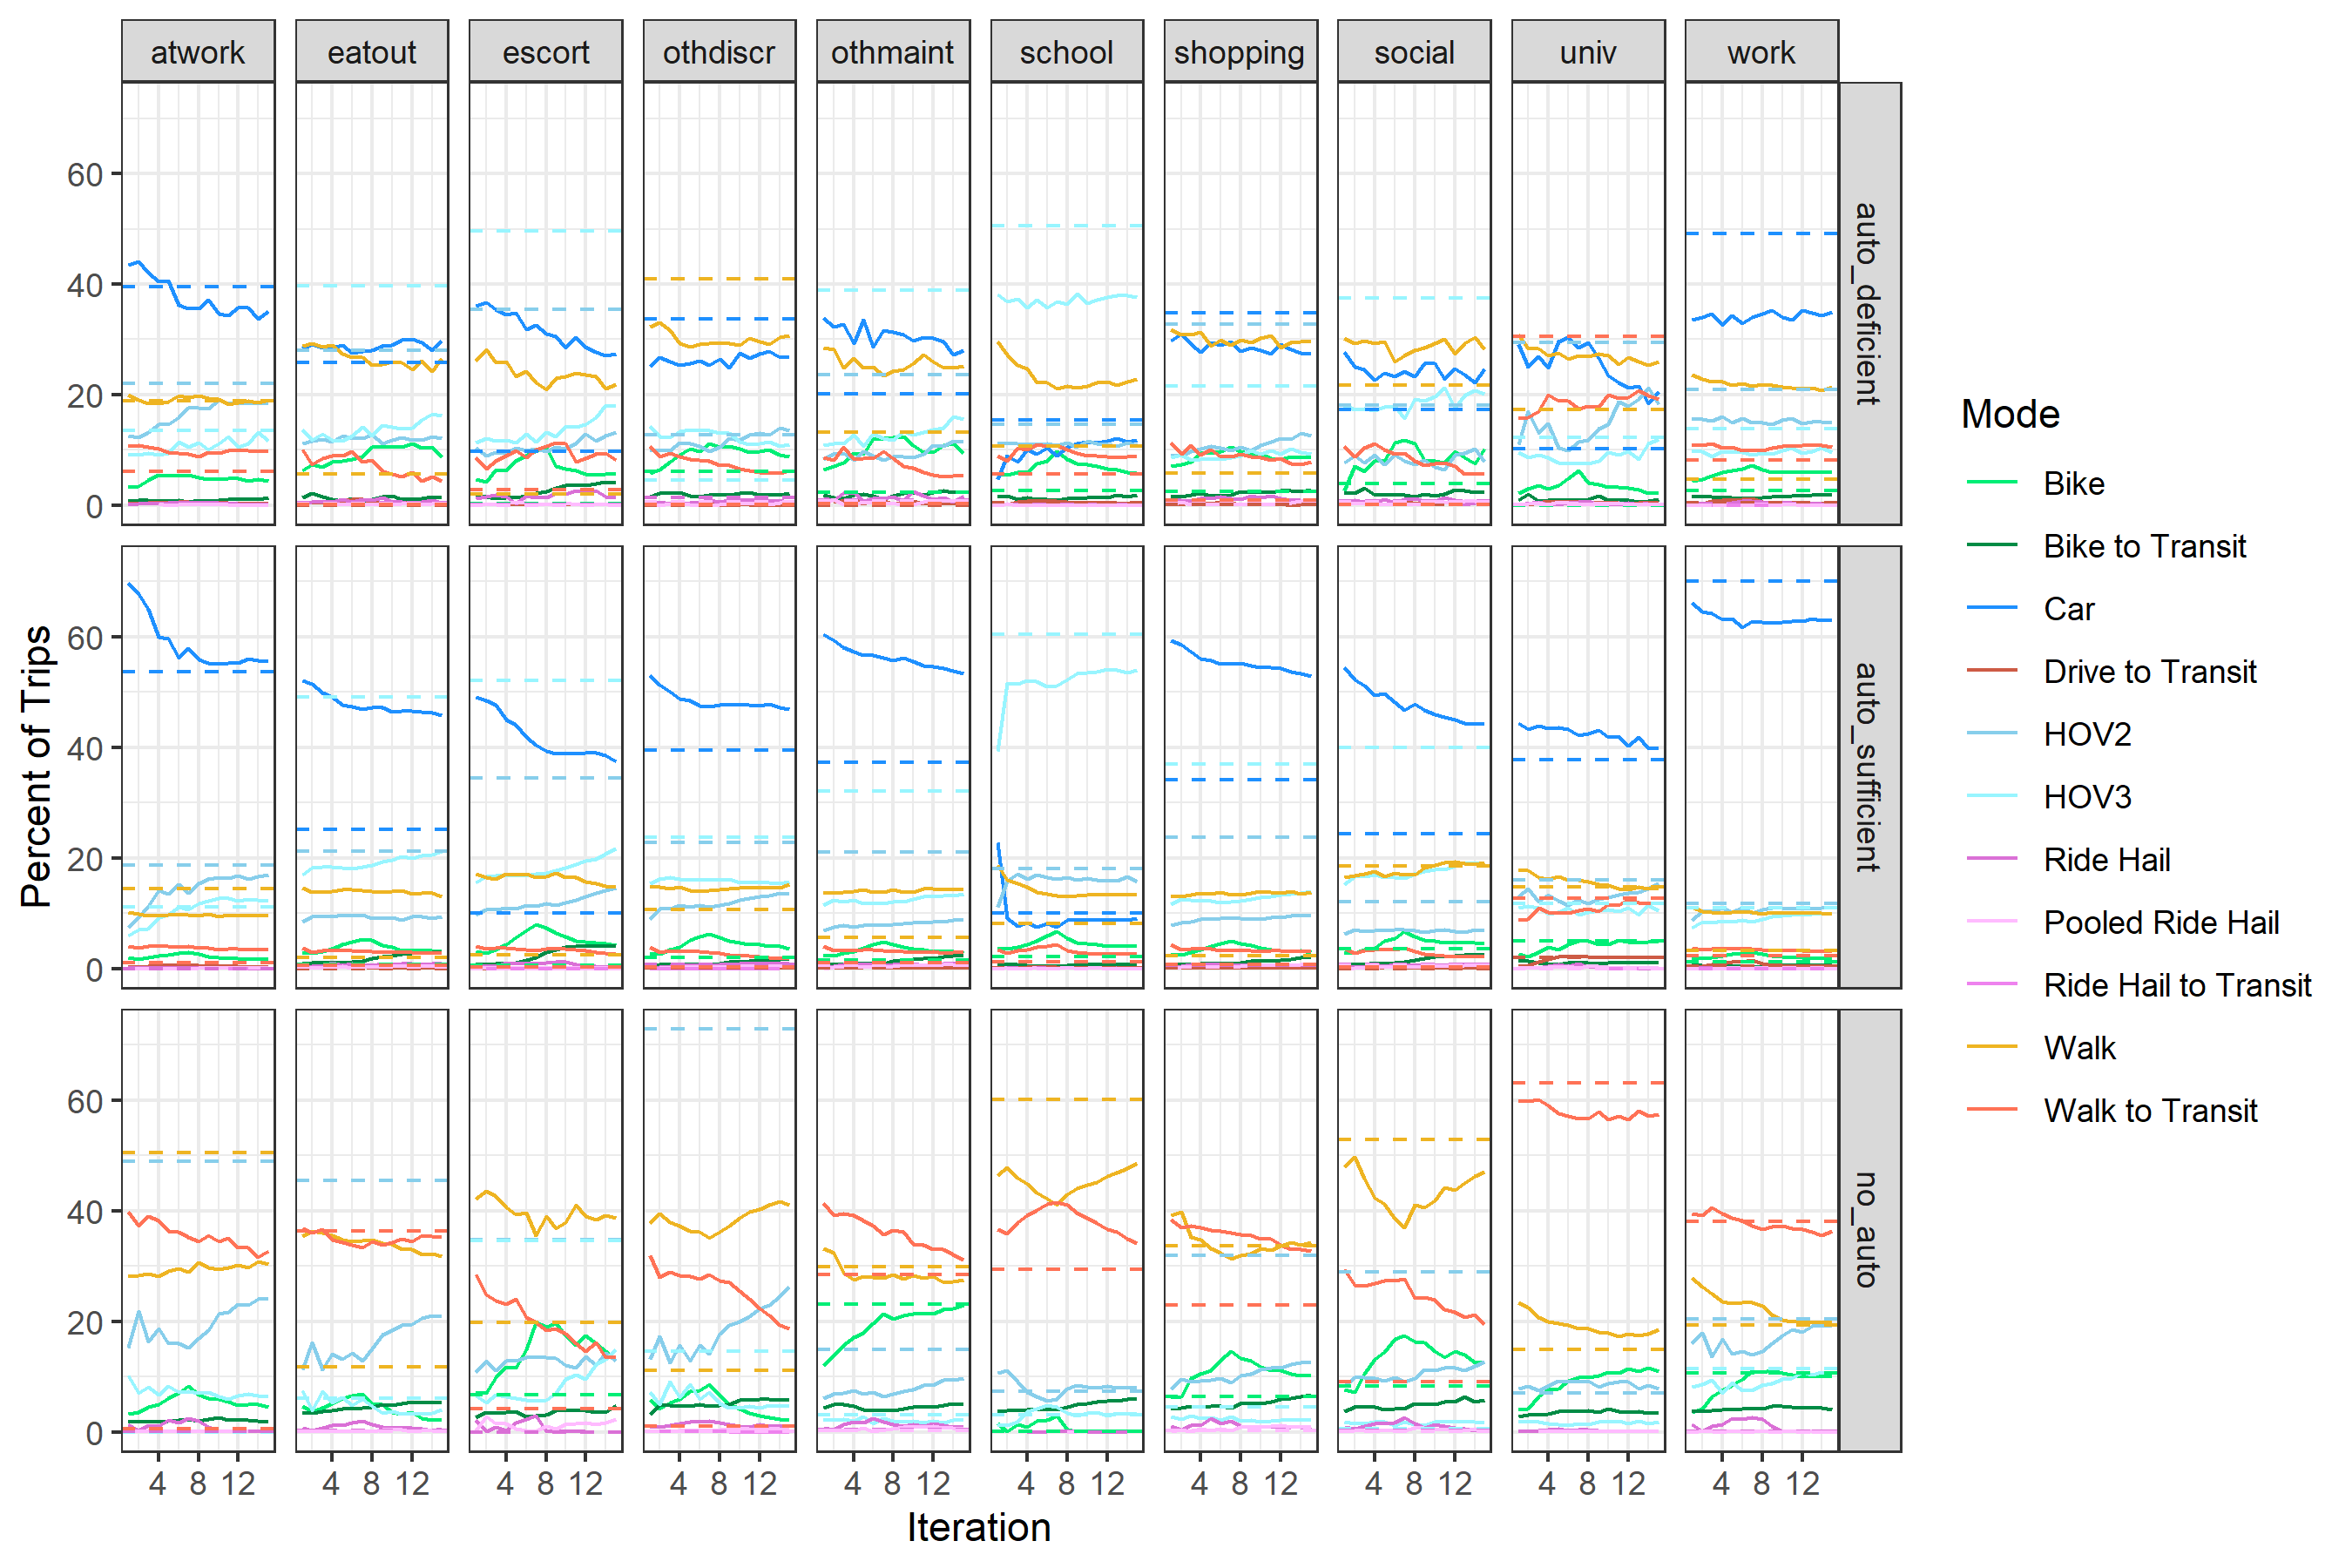
\includegraphics[width=1\linewidth]{pics/BeamCalib} 

}

\caption{BEAM mode choice ASC calibration.}\label{fig:fig-beam-calib}
\end{figure}

\hypertarget{meth-scenarios}{%
\section{Case Study Scenarios}\label{meth-scenarios}}

After BEAM validation and BEAM calibration were completed for the case study region, a series of different BEAM experiments were run. Each experiment was run for a total of 12 iterations using a 15\% population size. Ten different experiments were conducted, each with a unique ActivitySim-to-BEAM mode choice combination. Table \ref{tab:tbexperiments} provides a short name description of the 10 different scenarios.

\begin{table}
\caption{ActivitySim-to-BEAM Mode Choice Combination Scenario Names}
\renewcommand{\arraystretch}{2}
\[
  \begin{array}{cc|ccc}
    &\multicolumn{1}{c}{} & \multicolumn{2}{c}{\text{ActivitySim}} \\
    && \text{Plans without Ride Hail} & \text{Plans with RideHail}\\
    \hline
    & \text{None} & No RideHail & AsimRideHail \\
    \smash{\rotatebox[origin=c]{90}{\text{BEAM}}} & \text{RideHail} & \makecell{BeamRideHail:Path \\ BeamRideHail:PPL} & \makecell{AsimBeamRideHail:Path \\ AsimBeamRideHail:PPL} \\
    & \text{All} & \makecell{BeamAll:Path \\ BeamAll:PPL} & \makecell{AsimBeamAll:Path \\ AsimBeamAll:PPL}
  \end{array}
\]
\label{tab:tbexperiments}
\end{table}

To better describe the meaning of each scenario in Table \ref{tab:tbexperiments}, we explain the three mode choice descriptors that were altered in each scenario. The first descriptor references to how ActivitySim's modes were configured, which in Table \ref{tab:tbexperiments} is labeled under \emph{ActivitySim} as \emph{Plans without RideHail} and \emph{Plans with RideHail}. In the naming convention, any name starting with \emph{Asim} refers to any scenario where ride hail was included in the input plans from ActivitySim, and any name without \emph{Asim} refers to any a scenario where ride hail was excluded from the inputs plans from ActivitySim. To further explain, the ActivitySim ride hail nesting option as shown in Figure \ref{fig:fig-asim-nest} existed in one run of ActivitySim (\emph{Plans with RideHail}), whereas in the other it did not (\emph{Plans without RideHail}). Since the daily activity plans generated by ActivitySim were converted to BEAM inputs, this descriptor explains the initial mode choice selections for all trips entered into BEAM. By creating this distinction, we hope to better understand how heavily a multi-agent simulation prioritizes ride hail as opposed to an activity-based model.

The second descriptor present in Table \ref{tab:tbexperiments} is labeled under \emph{BEAM} as \emph{None}, \emph{RideHail}, and \emph{All}. These three variables explain which mode choice structure was used in BEAM. These variables also explain which modal alternatives were available for choice within BEAM. The \emph{None} category represents a run of BEAM where all modal innovation was turned off. This means that no mode choice was available, and the modes from the initial input plans remained constant across each iteration. This mode choice structure was used for the NoRideHail and AsimRideHail scenarios. The \emph{RideHail} category represented a run of BEAM where modal innovation was partially turned off. All trips that originally took car or carpool modes had modal innovation turned off; their modes were locked. All trips that originally took walk-transit or drive-transit modes, however, were given the option to switch to ride hail transit. Also, all walk modes were given the option to switch to ride hail. \emph{RideHail} represents the version of BEAM where ride hail and ride hail transit modes were only given to none-car dependent agents. The BeamRidehail and AsimBeamRideHail type scenarios implemented the \emph{RideHail} BEAM mode choice structure. Finally, the \emph{All} category represents a run of BEAM where modal innovation was turned on, and all modal alternatives were available for choice. This means that within-day replanning as well as across-day replanning was turned on, and agents could change their trip modes to maximize their utility. The BeamAll and AsimBeamAll type scenarios implemented the \emph{All} BEAM mode choice structure. Overall, by using different mode choice structures within BEAM, we hope to better understand how altering available modal alternatives affects ride hail service capabilities.

Finally, the third descriptor present in Table \ref{tab:tbexperiments} is labeled as either \emph{Path} or \emph{PPL} and explains which utility variables were used to calculate modal utility. Three different variations were present: \emph{Path}, \emph{PPL}, and empty. The empty option means no utility parameters were used in determining mode choice, because modal innovation as turned off completely. The \emph{Path} option represented the version of BEAM that only used path type utility parameters to calculate mode choice utility; location and person type variables were not used. The \emph{PPL} option represented the version of BEAM that used all utility parameter types (Path, Person, and Location) to calculate the mode choice utility. As ActivitySim uses path, person, and location type variables to determining modes, this version of BEAM also uses all three types of variables. Section \ref{meth-beam-link} describes how BEAM was configured to use all these variable types. By altering which variables were used in the utility equation, we hope to better understand the effect different types of utility parameters have on mode choice and ride hail service capabilities.

Overall, we ran 10 different scenarios each with a slightly different ActivitySim-to-BEAM mode choice combination. Each scenario is built from which modes were included in the input plans, which modal alternatives were available for choice, and which utility parameter types were used to calculate the mode choice utility. By altering these three different mode choice characteristics, we hope to better understand the affect a linked activity-based model and multi-agent simulation have on the service capabilities of a novel mode.

\hypertarget{results}{%
\chapter{Results}\label{results}}

We ran 10 different ActivitySim-to-BEAM mode choice combinations and processed their ride hail statistics and service capabilities into results. Specifically, we obtained ridership (Section \ref{res-ridership}) and wait time (Section \ref{res-waits}) information from the final iteration of BEAM for each scenario. Alongside each other, these results should shed some light on how differing mode choice structures between an activity-based model and a multi-agent simulation affect the forecasting of novel modes.

\hypertarget{res-ridership}{%
\section{Ridership}\label{res-ridership}}

As novel modes, like ride hail, become more popular it is ever more important to accurately predict ridership. Predicting accurate ridership totals will allow for efficient driver allocation, decreased traffic congestion, and improved rider experience (Chen et al., 2021). Table \ref{tab:ridership} shows the ridership percentages of ride hail, pooled ride hail, and ride hail transit modes for all 10 mode choice combinations. Correctly understanding the results of Table \ref{tab:ridership} may help forecasters predict ridership numbers more effectively in the future. To accurately interpret the results of Table \ref{tab:ridership} however, we must determine the best method to reading the table. The many slight variations in each mode choice structure makes interpreting the results complicated.

\begin{table}

\caption{\label{tab:ridership}Percent Ride Hail Ridership by Mode Choice Combination Scenario.}
\centering
\resizebox{\linewidth}{!}{
\begin{tabular}[t]{lrrrr}
\toprule
Scenario Name & Ride Hail & Pooled Ride Hail & Ride Hail to Transit & Total\\
\midrule
NoRideHail & 0.000 & 0.000 & 0.000 & 0.000\\
AsimRideHail & 0.024 & 0.003 & 0.000 & 0.027\\
BeamRideHail:Path & 3.814 & 2.120 & 0.249 & 6.183\\
BeamRideHail:PPL & 1.615 & 3.327 & 0.395 & 5.337\\
AsimBeamRideHail:Path & 1.824 & 3.465 & 0.461 & 5.750\\
\addlinespace
AsimBeamRideHail:PPL & 3.980 & 2.293 & 0.323 & 6.596\\
BeamAll:Path & 0.423 & 0.145 & 0.003 & 0.571\\
BeamAll:PPL & 0.280 & 0.567 & 0.011 & 0.858\\
AsimBeamAll:Path & 0.312 & 0.413 & 0.008 & 0.733\\
AsimBeamAll:PPL & 0.280 & 0.536 & 0.014 & 0.830\\
\bottomrule
\end{tabular}}
\end{table}

We propose two methodologies to interpreting the results of Table \ref{tab:ridership} as well as the other results presented in Section \ref{res-waits}.

\begin{enumerate}
\def\labelenumi{\arabic{enumi}.}
\tightlist
\item
  Comparing scenarios individually
\item
  Comparing scenarios collectively
\end{enumerate}

\hypertarget{res-ind}{%
\subsection{Comparing Scenarios Individually}\label{res-ind}}

To provide an example of using the first methodology, we compare the AsimRideHail scenario with the other nine scenarios. To begin, the AsimRideHail scenario compared with the NoRideHail scenario helps us understand how ActivitySim estimates ridership. Since the AsimRideHail scenario and NoRideHail scenario are run with BEAM's modal innovation turned off, we can assume that these results mimic those output from ActivitySim. Obviously the NoRideHail scenario will produce no ride hail results. Looking at the AsimRideHail scenario though, we clearly see the level at which ActivitySim predicts ridership. ActivitySim estimates that of the entire population's mode choice, 0.0024\% are ride hail modes, 0.003\% are pooled ride hail modes, and 0.000\% are ride hail transit modes. Since 0.000\% are ride hail transit trips, we conclude that ActivitySim may struggle at creating this particular mode option.

Comparing the AsimRideHail scenario with the \emph{RideHail} type scenarios (BeamRideHail and AsimBeamRideHail), less direct conclusions can be made. Of course, we obviously see that the ridership totals for all ride hail modes in all four scenarios are greater than the ridership of the AsimRideHail scenario. We can conclude that the BEAM mode choice structure which allows only ride hail modal innovation will predict higher ridership totals than ActivitySim. However, since each scenario presents a unique total ridership for each ride hail mode, we cannot draw any more conclusions by only referencing the results of the AsimRideHail scenario.

Comparing the AsimRideHail scenario with the BeamAll scenarios we see the effectiveness of BEAM at estimating ride hail modes without ride hail being selected in the initial plans. Both BeamAll scenarios display a large increase in total ride hail ridership when compared with the AsimRideHail scenario. Comparing the \emph{All} type scenarios (BeamAll and AsimBeamAll), we notice that BEAM will estimate higher ridership totals than ActivitySim, independent of whether or not the input plans include ride hailing modes. Comparing the AsimRideHail scenario with the BeamAll:Path and AsimBeamAll:Path scenarios we see a glimpse at how BEAM estimates ride hail modes with only path variables, independent of whether or not the input plans include ride hail. A significant increase in ridership in these two scenarios is displayed when compared with the AsimRideHail scenario. This may highlight the importance of including path variables to estimate ride hail ridership.

Finally, comparing the AsimRideHail scenario with the AsimBeamAll:PPL scenario we learn about the inter-workings of the BEAM mode choice that is most consistent with ActivitySim. The BeamAll:PPL and AsimBeamAll:PPL scenarios reference a BEAM mode choice structure which uses all modal options and all utility parameters. In other words, this BEAM mode choice structure is the one most aligned with that of ActivitySim. By comparing AsimBeamAll:PPL with the AsimRideHail scenario, we see how ride hail statistics \emph{differ} when modeled with an activity-based model than with a multiagent simulation. Looking at the differences between the the AsimRideHail and AsimBeamAll:PPL scenarios in Table \ref{tab:ridership}, we see an increase of 0.256\% of total ride hail modes, 0.533\% of total pooled ride hail, and 0.014\% of total ride hail transit modes. Overall, a significant increase in ridership was achieved by simply turning on modal innovation in BEAM. We conclude that BEAM is more prone to estimating higher ridership totals for ride hailing modes than ActivitySim.

Comparing other scenarios between each other individually may help us draw more conclusions, especially with the \emph{RideHail} type scenarios, however, analyzing every combination of individual scenario is beyond the extent of this paper. As a result, we instead move to comparing these scenarios collectively to better understand the ridership results.

\hypertarget{res-col}{%
\subsection{Comparing Scenarios Collectively}\label{res-col}}

Looking at scenarios collectively, and comparing them with each other and with other collective groups will extract deeper results in our research. Section \ref{meth-scenarios} and Table \ref{tab:tbexperiments} describe the following three different descriptors which will be used as the collective groups:

\begin{enumerate}
\def\labelenumi{\arabic{enumi}.}
\tightlist
\item
  ActivitySim Mode Choice / Input Plans
\item
  BEAM Mode Choice
\item
  BEAM Utility Variables
\end{enumerate}

As shown in Table \ref{tab:ridership}, minimal differences in ridership is produced between ActivitySim mode option outputs (scenarios with the \emph{Asim} prefix vs.~without). For example, comparing the \emph{RideHail} type scenarios we see no direct correlation with ridership and input plans. With the BeamRideHail:Path and AsimBeamRideHail:Path, we see that when ride hail doesn't exist in the input plans, the total ride hail type modes (ride hail, pooled ride hail, and ride hail transit) complete about 6.2\% of total modal distribution whereas when ride hail type modes are included, total ride hail type modes complete about 5.8\% of total modal distribution. Although both project an enormous share using ride hail, the scenario with ride hail in the input plans projects more ride hail ridership. Oddly enough, however, when comparing the BeamRideHail:PPL and AsimBeamRideHail:PPL scenarios, the scenario with ride hail in the input plans projects less ride hail ridership. In these two scenarios we see that when ride hail doesn't exist in the input plans, the total ride hail type modes complete about 5.3\% of total modal distribution whereas when ride hail type modes are included, total ride hail type modes complete around 6.6\% of total modal distribution. Overall, no direct correlation between ride hail ridership totals and input plans is seen between \emph{RideHail} type scenarios. Then, when examining BeamAll:PPL and AsimBeamAll:PPL, the output ridership percentages are almost identical. When using the BEAM mode choice model that is most consistent with that of ActivitySim, BEAM estimates ride hail ridership at the same level with or without ride hail in the input plans. However, when examining BeamAll:Path and AsimBeamAll:Path we see that when only path variables are used in the utility equation, ridership is not identical between ActivitySim mode options. BeamAll:Path shows an increase in ridership for ride hail modes and a decrease in pooled ride hail and ride hail transit modes than in AsimBeamAll:Path. Initial plan sets play a role in who selects pooled and transit ride hail trips when only using path variables to determine mode choice. We hypothesize that with the lack of person attributes in the utility equation, pooled and transit ride hail options look less appealing. Collectively, comparing Scenarios AsimRideHail, AsimBeamRideHail:Path, AsimBeamRideHail:PPL, AsimBeamAll:Path, and AsimBeamAll:PPL against Scenarios NoRideHail, BeamRideHail:Path, BeamRideHail:PPL, BeamAll:Path, and BeamAll:PPL we see similar results among similar mode choice structures. Although minimal shifts in total ridership were noticed in most cases, as a whole, we determine that changing the ActivitySim mode options has no \emph{significant} change in final ride hail ridership; at least not a traceable change.

However, when analyzing the BEAM mode options from Table \ref{tab:ridership} as described in Table \ref{tab:tbexperiments}, obvious results are seen. The \emph{None} type scenarios (NoRideHail and AsimRideHail) produce little to no agents choosing ride hail. The reasoning behind this is described in Section \ref{res-ind}. On the other hand, the \emph{RideHail} type scenarios (BeamRideHail and AsimBeamRideHail) produce the largest number of ride hail modes amoung BEAM mode choice structures! This is because with the \emph{RideHail} type mode choice, walking individuals only have the option to continue walking or take ride hail. Taking a ride hail mode is usually more attractive than walking a long distance; and because of this limitation, an excessive number of agents switch to using ride hail. Finally, the \emph{All} type scenarios (BeamAll and AsimBeamAll) produce a significantly larger number of ride hail modes than the \emph{None} type. According to BEAM, ride hail type modes are more attractive than initially projected by ActivitySim. Ridership is affected significantly by which mode choice structure is used by BEAM; this conclusion is clear.

Finally, we can analyze the effect the BEAM utility variables have on ride hail ridership totals. Two different options are shown: Path and PPL. To best understand the effect the utility variables have, we compare similar BEAM structures with the utility variables adjusted. For example, BeamRideHail:Path and BeamRideHail:PPL can be compared together. In this case, the ride hail ridership decreases (3.814\% to 1.615\%) when using path, person, and location variables, but increases with pooled ride hail (2.120\% to 3.327\%) and ride hail transit (0.249\% and 0.395\%) when using path, person, and location variables. This same pattern occurs when analyzing the difference between the BeamAll:Path and BeamAll:PPL, and AsimBeamAll:Path and AsimBeamAll:PPL scenarios. For some oddity, AsimBeamRideHail:Path and AsimBeamRideHail:PPL follow an opposite pattern where ride hail increases (1.824\% to 3.980\%) and ride hail pooled decreases (3.465\% to 2.293\%) and ride hail transit decreases (0.461\% to 0.323\%) when using path, person, and location variables. Similarly, with all comparisons except between BeamRideHail:Path and BeamRideHail:PPL, we see that total ride hail percentages increases when using all path, person, and location variables to estimate ride hail. We acknowledge that not all scenarios follow the same pattern, but conclude that in general, using only path variables to estimate ride hail ridership will result in less total ride hail ridership than if using all path, person, and location type variables.

\hypertarget{summary}{%
\subsection{Summary}\label{summary}}

Analyzing ridership among different mode choice structures has highlighted some important conclusions:

\begin{itemize}
\item
  Ride hail is affected significantly by which mode choice structure is used by BEAM.

  \begin{itemize}
  \item
    The \emph{RideHail} BEAM mode structure will estimate much more ride hail usage than the other versions.
  \item
    The \emph{All} BEAM mode structure is prone to estimating higher ride hail usage than ActivitySim.
  \end{itemize}
\item
  Initial plans, and whether or not they include ride hail, do not significantly affect the level at which BEAM estimates ride hail.
\item
  Path variables affects ridership; and using all path, person, and location type variables will increase total ridership.
\item
  With the lack of person attributes in the utility equation, pooled and transit ride hail options look less appealing.
\end{itemize}

By analyzing wait times with a similar approach, individually and collectively, many of these conclusions are verified.

\hypertarget{res-waits}{%
\section{Wait Times}\label{res-waits}}

Wait time is one of the most important factors people use when determining their travel mode. When traveling, long wait times are seen as burdensome; short wait times are also seen as burdensome when compared to modes with zero wait time. Therefore, estimating accurate wait times would be helpful to forecasters in understanding the usage of novel modes. Ride hail, in particular, is an up and coming novel mode where wait time definitely plays a factor in its usage. According to Dong (2020), wait time for ride hailing modes seems less burdensome than wait time for transit modes. This behavior may lead to higher ridership for ride hail vehicles than for transit vehicles. Since ridership hinges on wait time among other things, the accurate estimation of wait times (and other service capabilities) in essential to forecasting novel modes like ride hail.

Figure \ref{fig:waits} shows the results of wait times for ride hail vehicles for the scenarios that were run. (The NoRidehail scenario, is not shown because no ride hail vehicles were present in that scenario). By analyzing the wait times with violin plots, we analyze a detailed distribution of the ride hail wait times for each scenario.

\begin{figure}

{\centering 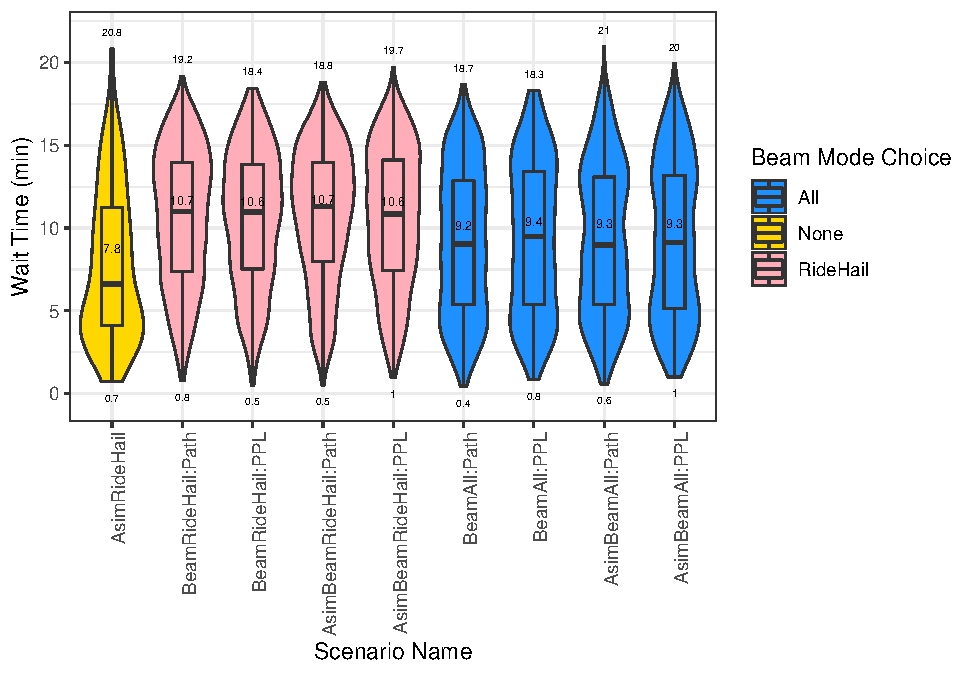
\includegraphics{thesis_files/figure-latex/waits-1} 

}

\caption{Distribution of ride hail wait times by mode choice combination scenario.}\label{fig:waits}
\end{figure}

\hypertarget{comparing-scenarios-individually}{%
\subsection{Comparing Scenarios Individually}\label{comparing-scenarios-individually}}

As was done in Section \ref{res-ind}, we compare some scenarios individually with each other. To start, we look at the differences that exist between AsimRideHail and AsimBeamAll:PPL. As explained when looking at ridership, this comparison explains the inter-workings of the BEAM mode choice model that is most consistent with ActivitySim. As ridership experiences an increase between these two scenarios, wait times also increase when using the BEAM mode choice model (minimum wait time increases from 0.7 to 1 minute, and mean wait time increases from 7.8 to 9.3 minutes). A noticeable increase in wait time was achieved by simply turning on modal innovation in BEAM. Since higher wait time suggest higher ridership, we again conclude that BEAM is more prone to estimating more ride hail usage than ActivitySim.

Comparing AsimRideHail and BeamAll:PPL we see the lack of impact that ride hail in the initial plans has on effective ride hail usage. The wait time mean may have increased from 7.8 to 8.4 minutes, but the maximum wait time decreased from 20.8 to 18.3 minutes! Although no ride hail existed in the input plans, BEAM was effectively able to calculate the usage of more ride hail vehicles with less maximum wait times. Comparing AsimRideHail with BeamAll:Path and AsimBeamAll:Path, we can learn of the effect using only Path variables has on wait time. In both BeamAll:Path and AsimBeamAll:Path, mean wait time increases when compared with AsimRideHail, but AsimBeamAll:Path displays a larger maximum wait time than BeamAll:Path and AsimRideHail. This may highlight the importance of also using person and location variables to estimate ride hail wait time. The individual comparisons between AsimRideHail and the \emph{RideHail} type scenarios are not included in this analysis, but can be personally examined using the same technique.

\hypertarget{comparing-scenarios-collectively}{%
\subsection{Comparing Scenarios Collectively}\label{comparing-scenarios-collectively}}

As with ridership, analyzing wait times on a collective scale sheds additional light in the effect mode choice has on ride hail service capabilities. To start we analyze the effect the input plans have on ride hail wait times. Collectively, comparing the scenarios with the \emph{Asim} prefix against the scenarios without, we see a slight difference in maximum wait times. For example, Scenarios AsimBeamRideHail:PPL, AsimBeamAll:Path, and AsimBeamAll:PPL have higher maximum wait times when compared to their counterparts in BeamRideHail:PPL, BeamAll:Path, BeamAll:PPL. Although this is true, when comparing the mean values of those same scenarios, relatively no difference exists. Its hard to conclude the exact effect that having ride hail in the input plans has, but we propose a hypothesis. We suppose that the existence of ride hail in the initial plans will not affect \emph{most} ride hail wait times. With the exception of the maximum value, similar wait time distributions and means exist between different input ride hail wait times. The presence of ride hail in the input plans may, however, affect those few riders who start with ride hail in their input plans; maybe they are the users with longer wait times. There is insufficient data to conclude this though, and even so, the majority of wait time calculations are not affected. As concluded by analyzing ridership values, as a whole we determine that changing the ActivitySim mode options creates insignificant changes in the final ride hail performance in BEAM.

Alternately, comparing different BEAM mode options does significantly affect ride hail wait times. The \emph{None} type scenario (AsimRideHail) has the largest spread of wait times, the lowest mean wait time, and is ``bottom heavy'' -- referring to the fact that a major cluster of users wait less than 7.5 minutes. The \emph{All} type scenarios have higher mean wait times (\textasciitilde9.3 minutes) than the \emph{None} type and lower mean wait times than the \emph{RideHail} type. Neither top nor bottom heavy, the \emph{All} type scenarios seem to have a more even spread in wait times, ranging from 0.4 to 21 minutes (depending on the exact mode choice structure). BEAM seems to paint ride hail alternatives as more desirable than ActivitySim, as more users are willing to wait longer (12 to 18 minutes in the \emph{All} scenarios). This is especially true with the \emph{RideHail} type scenarios, as these scenarios are the most ``top heavy'' in comparison; a large cluster of users are willing to wait 7.5 to 20 minutes. The \emph{RideHail} type scenarios have the largest mean wait times (\textasciitilde10.65 minutes). Overall, wait time is significantly affected by which mode choice structure is used by BEAM, just like as was concluded with ridership.

The last group to compare collectively is between the Path and PPL models. By comparing BeamRideHail:Path and BeamRideHail:PPL, BeamAll:Path and BeamAll:PPL, and AsimBeamAll:Path and AsimBeamAll:PPL, we see that the Path models estimate a slightly higher maximum wait time. In addition, BeamRideHail:Path and AsimBeamRideHail:Path seem to have a larger cluster above a 10 minute wait time than BeamRideHail:PPL and AsimBeamRideHail:PPL. Besides these two observations though, the differences between utility parameters is minimal Although ridership was affected by which utility parameters were used, wait time is only slightly affected. We conclude that by lacking person and location variables, there is potential for a longer wait time for ride hail vehicles, although this observation is not concrete. More research would need to be done on this subject that is not within the scope of this paper.

\hypertarget{summary-1}{%
\subsection{Summary}\label{summary-1}}

Overall, by analyzing ride hail wait times we saw many of the same conclusions drawn by the ridership percentages verified. Ride hail service capabilities is affected significantly by the mode choice structure chosen. Initial plan, and whether or not they include ride hail, does affect service capabilities but only minimally (potential for longer wait times). Finally, the utility parameters used to calculate the mode choice does affect ridership. Ridership will increase when person and location variables are included. There is also potential for longer wait times when those variables are not included. These conclusions are clear, however, much of the results can be further explained by things beyond our control within this study. Section \ref{deep-look} takes a deeper look at why some patterns in the ridership and wait times results exist.

\hypertarget{deep-look}{%
\section{A Deeper Look at Ridership and Wait Times}\label{deep-look}}

The results from Table \ref{tab:tbexperiments} and the results from Figure \ref{fig:waits} can be explained further by understanding the original setup of the experiments. For example, the clearest distinction in ridership and wait times exist between BEAM mode choice structures. The \emph{None}, \emph{RideHail}, and \emph{All} structure types each produce results at a different magnitude. These vastly different results are directly related to how each model structure was constructed. To best explain the structure of each type however, Section \ref{type1} fist explains the \emph{None} structure, Section \ref{type3} then explains the \emph{All} structure, and finally Section \ref{type2} explains the \emph{RideHail} structure. The \emph{All} structure is more complex than the \emph{RideHail} structure, but the \emph{RideHail} structure was constructed in part due to the problems within the \emph{All} structure. For this reason, we explain the \emph{All} structure before the \emph{RideHail} structure.

\hypertarget{type1}{%
\subsection{BEAM (None) Effect on Results}\label{type1}}

The \emph{None} BEAM mode choice model type uses no mode choice code from the BEAM software. As explained in Table \ref{tab:tbexperiments}, this scenario descriptor points toward turning off BEAM's modal innovation. In a way, the results from these scenarios are almost identical to the direct output of ActivitySim itself. Since BEAM locked every trip's mode selection, we used these experiments to help understand the difference between how BEAM estimates ride hail against how ActivitySim estimates ride hail. Although it may seem illogical to use BEAM on top of ActivitySim for the \emph{None} type scenarios, it was still necessary to run them with BEAM because BEAM estimates ride hail service capabilities with more detail than ActivitySim (See Section \ref{lit-mas}).

\hypertarget{type3}{%
\subsection{BEAM (All) Effect on Results}\label{type3}}

The \emph{All} BEAM mode choice model type uses a linked mode choice model with that of ActivitySim (See Section \ref{meth-beam-link}) with all modal alternatives available. This adjusted model structure helps us better understand why we obtained much higher ridership than with the \emph{None} type. Figure \ref{fig:piechart} shows from which modes agents who switched to ride hail came from. Interestingly enough, the majority of agents who select ride hail switched from car type modes (Car, HOV2, HOV3). Adding together the car type modes, 74\% of agents from the AsimBeamAll:Path scenario, 73\% from the AsimBeamAll:PPL scenario, 74\% of agents from the BeamAll:Path scenario, and 75\% of agents from the BeamAll:PPL scenario switch from a car type mode to a ride hail type mode by the last iteration. While about three-fourths of agents switch to ride hail from car type modes, 14-17\% of agents switch from walk modes. Why is it that the \emph{All} BEAM mode choice structure projects that the majority of ride hail users originate from car type modes? The \emph{All} mode choice structure is consistent with that of ActivitySim, yet 75\% of ride hail users go against ActivitySim's original mode choice selection to use a car type vehicle.

\begin{figure}

{\centering 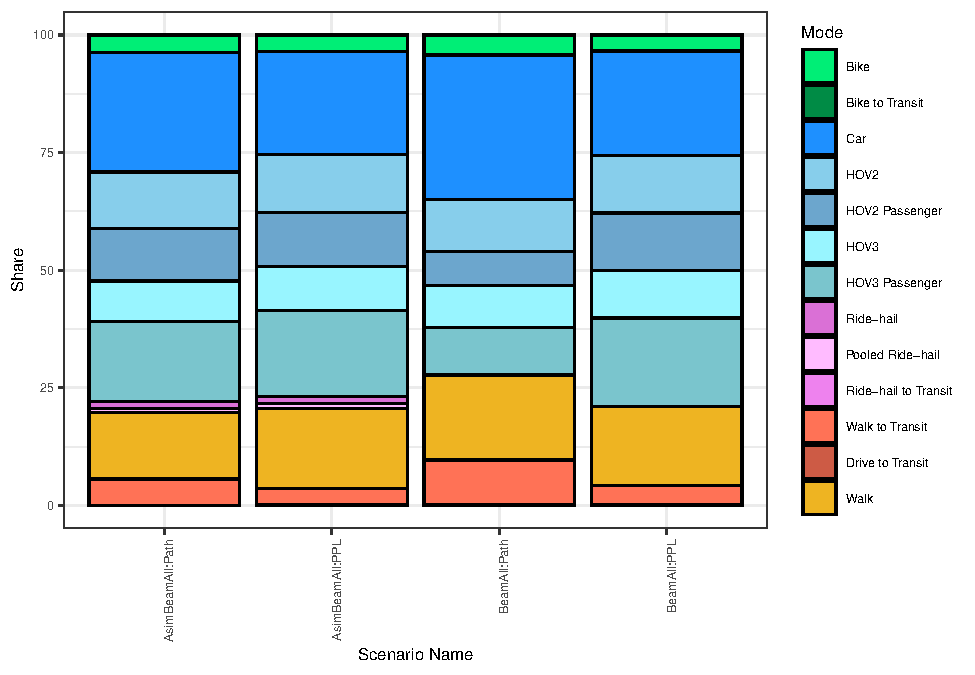
\includegraphics{thesis_files/figure-latex/piechart-1} 

}

\caption{Original mode choices of agents who switch to a ride hail type mode.}\label{fig:piechart}
\end{figure}

We offer two factors as to why so many car users switch to ride hail modes. The first is that with the consistent mode choice structure, new utility parameter values are used to calculate the mode choice utility. The new utility parameters boost the ride hail utility, turning ride hail options into attractive alternatives. Figure \ref{fig:sankey} provides sufficient evidence for this claim. Figure \ref{fig:sankey} shows a sankey diagram of all modal decisions at the start of each iteration for the AsimBeamAll:PPL scenario. The mode ``No Mode'' describes those modes that were cleared and reset at the beginning of each iteration. (\textasciitilde10\% of all trips had their modes reset each iteration). Notice how many of the Car, HOV2, HOV2 Passenger, HOV3, and HOV3 Passenger modes shift into the ``No Mode'' category each iteration. Also notice in the subsequent iteration how many of those ``No Mode'' choices shift to ride hail modes! A shift from the ``No Mode'' choice to ride hail represents those agents choosing their mode based on the utility value.

\begin{landscape}

\begin{figure}[H]
\centering
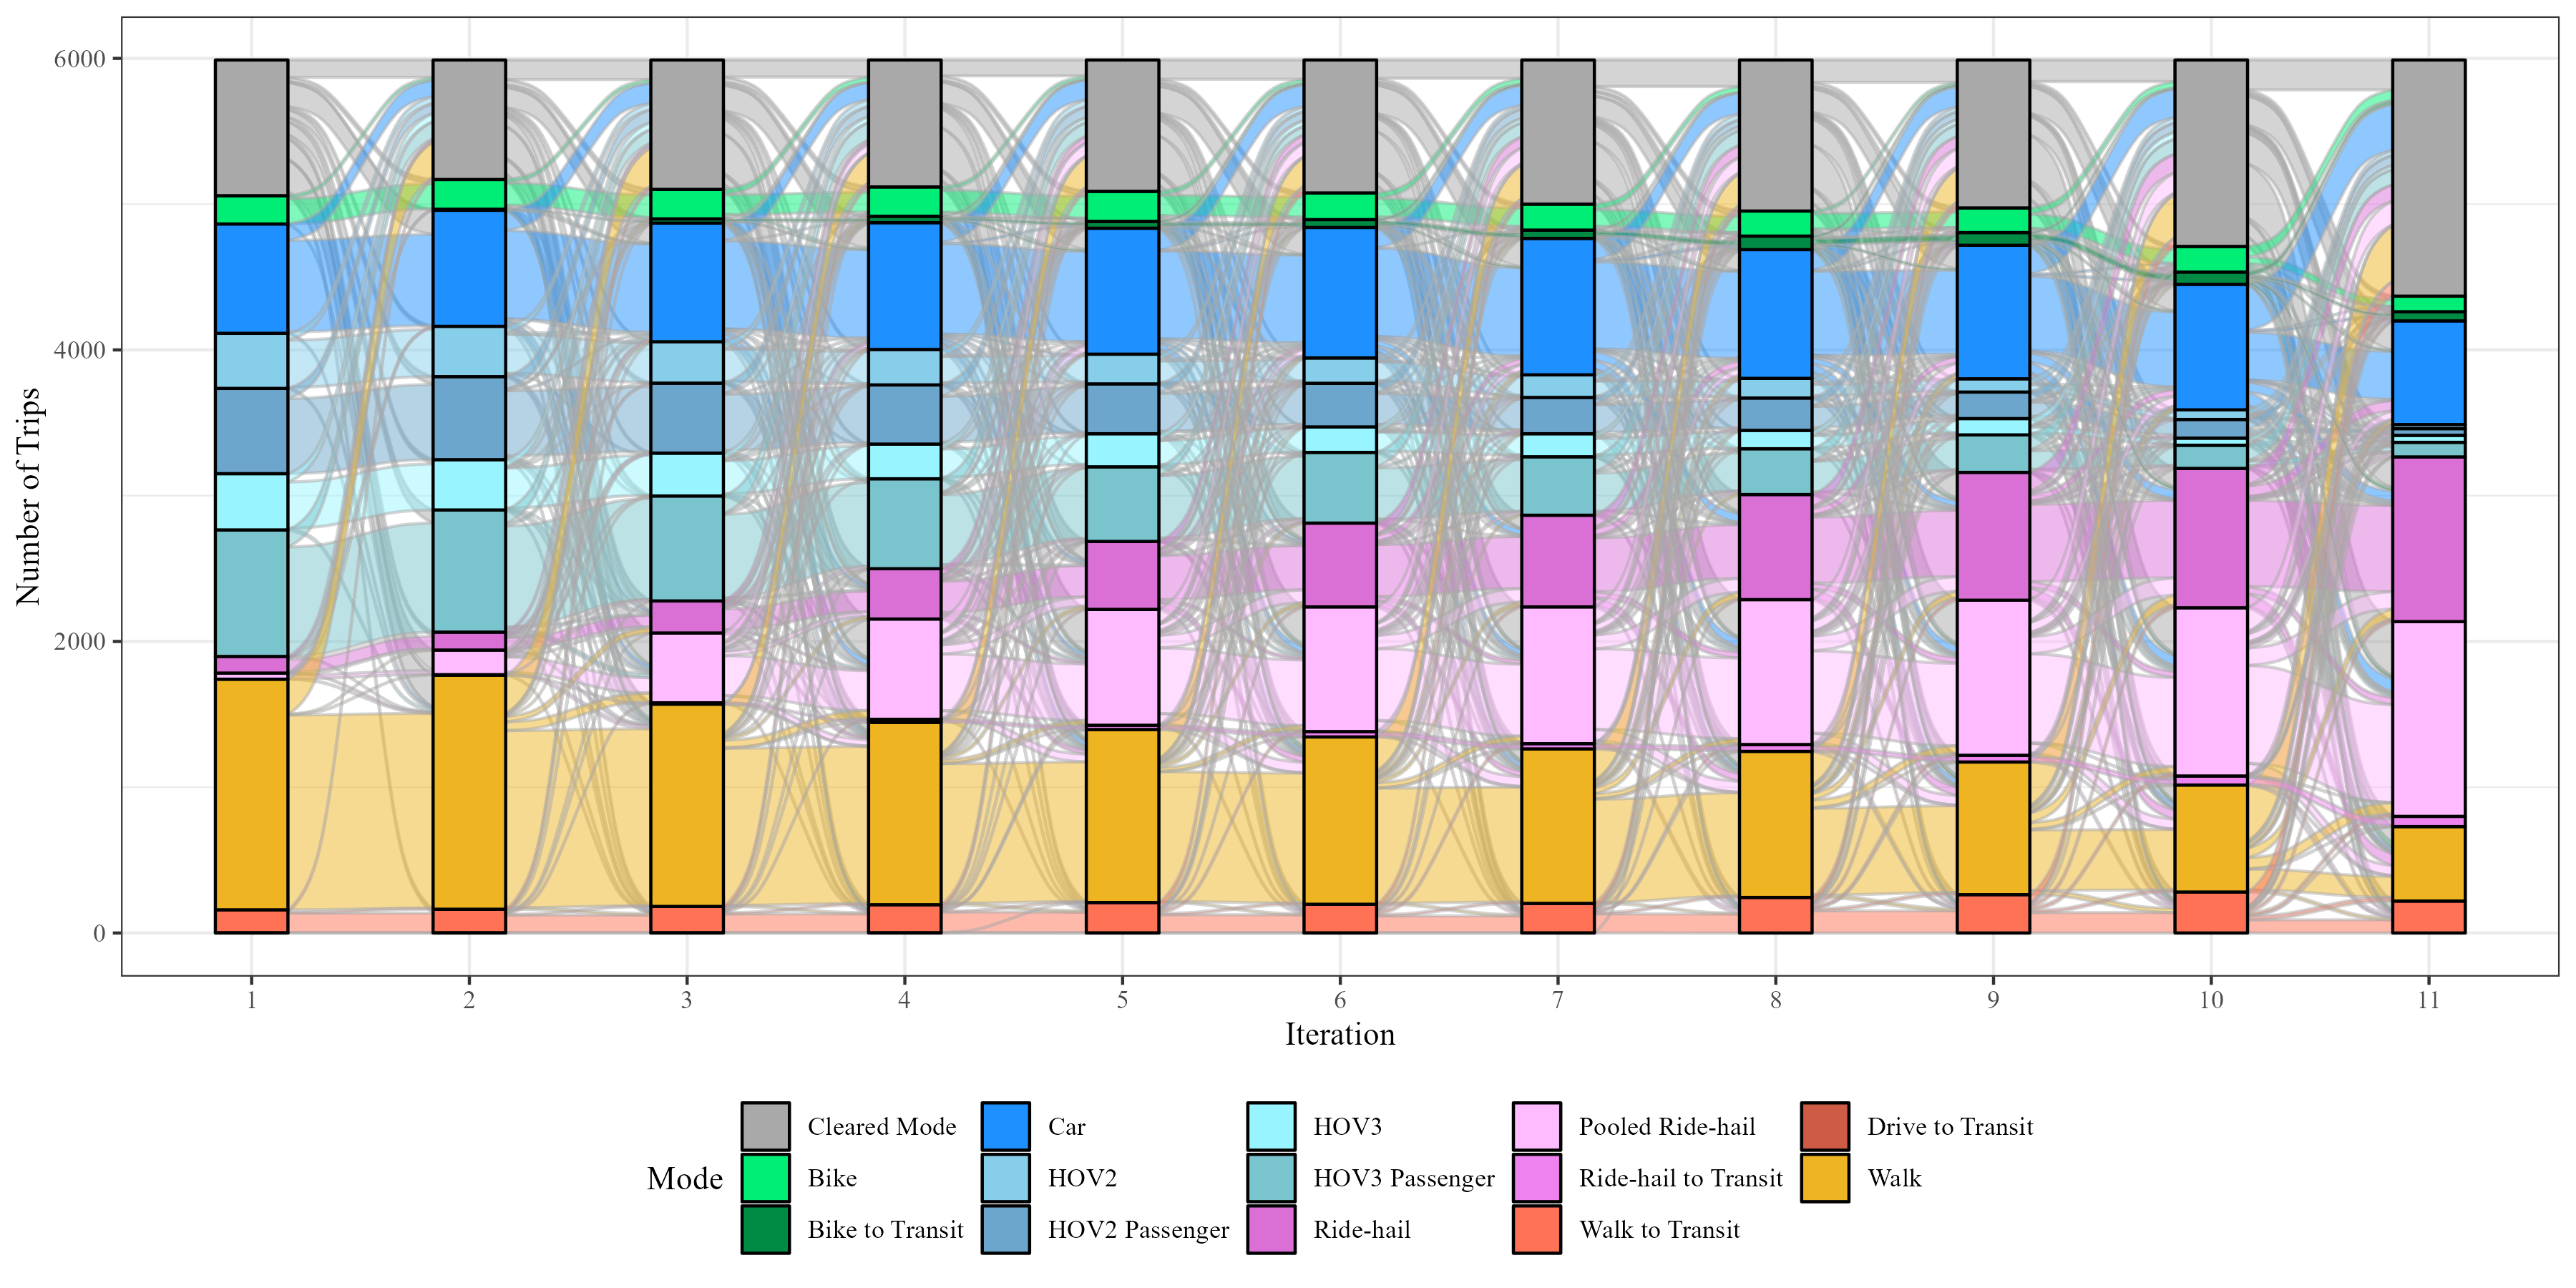
\includegraphics{planshifts.png}
\caption{The entire selection process of agents who use ride hail on the final iteration.}
\label{fig:sankey}
\end{figure}

\end{landscape}

The second factor for why agents switch from car to ride hail has to do with how BEAM is programmed. BEAM implements a complex car tracking algorithm which keeps track of household and agent level vehicle allocation. For example, if a household owns one vehicle, then the vehicle is \emph{assigned} to the first agent to use it in their daily plan. This leaves the other household members to choose an alternate mode. ActivitySim monitors vehicle and agent level vehicle allocation differently by using auto sufficiency to estimate car mode choice at the household level. (Auto sufficient households are more likely to choose car than auto deficient households). BEAM's implementation of vehicular assignment prevents many agents from selecting a car mode, whereas ActivitySim may not prevent those same individuals from car usage. In addition to BEAM's vehicle assignment algorithm, BEAM's trip based mode choice structure also forces some car users to switch modes. Sometimes, agents will \emph{lose} their vehicle within the day. This occurs when a pathway cannot be built. If an agent \emph{loses} their car, they are likely to become unable to choose the car mode on future trips, as the car is usually gone and is no longer a valid modal alternative. Figure \ref{fig:walkers} provides evidence for this statement. Figure \ref{fig:walkers} displays a graph of those agents who start their day using a mode other than walk, but end up switching to the walk mode by the end of the day for the AsimBeamAll:PPL scenario. Notice how in each hour, as the percentage of walk users increases the percentage of car type modes remains constant or decreases. This helps show that hundreds of car type mode users are switching to walk modes instead of remaining with their vehicle. Choosing walk on a car tour usually means the car path couldn't be built and the car is unable to be used on future trips within the day. Looking at Figure \ref{fig:sankey} again, we notice that many walk users shift to ride hail each iteration. Therefore, many car type users who shift to walk during one trip, may shift to ride hail type vehicles on the next trip. This is true between corresponding iterations as well.

\begin{figure}

{\centering 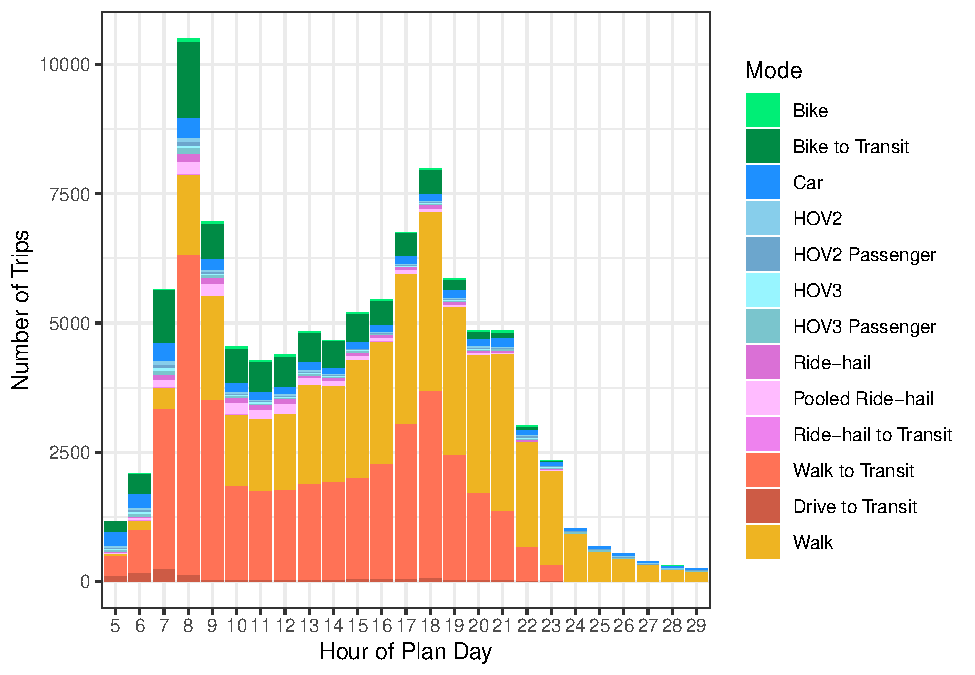
\includegraphics{thesis_files/figure-latex/walkers-1} 

}

\caption{Agents who switch to walk by time of day.}\label{fig:walkers}
\end{figure}

Overall, BEAM's internal code structure creates reasons to be unable to choose car modes, forcing agents to switch modal alternatives or get assigned the walk mode. The increase in ridership in the \emph{All} model from the \emph{None} model can be partially explained for these reasons.

\hypertarget{type2}{%
\subsection{BEAM (RideHail) Effect on Results}\label{type2}}

Finally, the way the \emph{RideHail} BEAM mode choice model was constructed explains why their ridership and wait times were high. The \emph{RideHail} model uses a linked mode choice model with that of ActivitySim, but only walk and transit users have the option to switch to ride hail type modes; car-type modes remained locked across each iteration. Whenever a ride hail path could be built, all walk modes were automatically given the option to choose ride hail or ride hail pooled and all transit modes were automatically given the option to choose ride hail transit. Although it made logical sense to lock all car-type modes (for reasons described in Section \ref{type3}), by giving ride hail options only to walk and transit users, ridership increased even more than in the \emph{All} scenario. The increase in ridership occurred because 1.) BEAM's adjusted code forced ride hail to be an option in almost all cases, and 2.) in most cases ride hail was calculated to be more attractive than walk or transit modes.

Table \ref{tab:timeutil} provides evidence in ride hail being an attractive mode choice alternative. Table \ref{tab:timeutil} displays the ride hail time utilization for each of the scenarios performed (except for NoRideHail). The same ride hail fleet was used in each of the nine scenarios. The ride hail fleet was composed of 952 ride hail driver shifts. Ride hail time utilization was calculated as the sum of all the driver shift times divided by the sum of all the passenger occupied ride hail travel time. Obviously, the AsimRideHail scenario had the lowest ride hail time utilization, at only 4.046\%. This was because ActivitySim estimated a low ride hail ridership percentage and more drivers existed than riders. Interestingly, the \emph{All} type scenarios ranged from 53.123\% to 62.459\% ride hail time utilization. This explains the higher wait times shown in Figure \ref{fig:waits}! Higher ride hail utilization also explains why the Path models had higher maximum wait times. Finally, by analyzing the ride hail time utilization for the \emph{RideHail} scenarios, we fully understand how attractive ride hail was. With 70.270\% to 73.777\% of ride hail time utilization present for the \emph{RideHail} scenarios, we see three fourths of each driver's shift was used to transport passengers. This explains the attractiveness of the choice, the extreme increase in ridership, and also the increased wait time for the \emph{RideHail} type scenarios. In addition, it shows that if more driver shifts were available for the \emph{RideHail} scenarios, wait times would have been lower and ridership would have been higher.

\begin{table}

\caption{\label{tab:timeutil}Percent Ride Hail Time Utilization by Mode Choice Combination Scenario}
\centering
\begin{tabular}[t]{lr}
\toprule
ScenarioName & RideHailTimeUtilization\\
\midrule
AsimRideHail & 4.046\\
BeamRideHail:Path & 73.777\\
BeamRideHail:PPL & 70.270\\
AsimBeamRideHail:Path & 71.354\\
AsimBeamRideHail:PPL & 72.590\\
\addlinespace
BeamAll:Path & 62.459\\
BeamAll:PPL & 53.143\\
AsimBeamAll:Path & 58.739\\
AsimBeamAll:PPL & 53.123\\
\bottomrule
\end{tabular}
\end{table}

\hypertarget{summary-2}{%
\subsection{Summary}\label{summary-2}}

As seen by the explanation of the structure of the \emph{None}, \emph{All}, and \emph{RideHail} type scenarios, how BEAM's different mode choice structures are programmed affected total ride hail ridership and wait times significantly. By examining these structural differences, we better understand the effect mode choice has on forecasting novel modes. For example, the use of path, person, and location type variables cause ride hail to be a more attractive choice than if it were only calculated with the default BEAM parameters (See Section \ref{novel-beam}). In addition, BEAM's advanced car tracking algorithm and trip based mode structure causes many car type trips to shift to ride hail after first defaulting to the walk mode. Finally, we conclude that the \emph{RideHail} type scenario is best at forecasting novel mode usage, as shown by the high ride hail time utilization percentages. The \emph{RideHail} type scenario also avoids the BEAM pitfalls of loosing car modes and provides ride hailing vehicles to those who need it most. Although this is true, its limitation exists in that \emph{all} walk trips are given the option to shift to ride hail. In reality, only those walk trips who get their mode choice cleared after each iteration should have the opportunity to switch modes. This was not accounted for in the research methodology because of the complexity of the BEAM code adjustment. Section \ref{discussion} further describes the deeper meaning behind the ride hail, wait time, and mode choice structure results discovered in this section.

\hypertarget{discussion}{%
\chapter{Discussion}\label{discussion}}

According to the results presented in Section \ref{results}, mode choice structure significantly affects novel mode ridership and service capabilities. The results also suggest that whether or not ride hail exists in the multi-agent simulation's input plans does not make a significant difference to overall ride hail statistics. With both of these determinations in mind, we conclude that forecasters should use \emph{both} an activity-based model and a multi-agent simulation to forecast novel mode usage. However, we suggest that only one of these tools should be used to forecast ridership, while the multi-agent simulation should be used to forecast service capabilities. The results, backed up by the literature review conducted in Section \ref{lit}, illustrate why the multi-agent simulation should be used for service capability estimation. The results also suggest why only one of the tools should be used for ridership estimation. Specifically, the extreme variation in ridership among the 10 scenarios supports this conclusion. Overall, with these conclusions in mind, we offer two methodological approaches that forecasters should use to model novel modes:

\begin{enumerate}
\def\labelenumi{\arabic{enumi}.}
\tightlist
\item
  Frozen Multi-Agent Estimation
\item
  Adjusted/Enhanced Multi-Agent Estimation
\end{enumerate}

\hypertarget{frozen-multi-agent-estimation}{%
\section{Frozen Multi-Agent Estimation}\label{frozen-multi-agent-estimation}}

In the Frozen Multi-Agent Estimation technique, we advice forecasters to use an activity-based model to estimate novel mode ridership usage. The activity-based model would be in charge of forecasting which users are prone to using the new mode and how many of these users should exist. Then, we advice forecasters to input these final plans into a multi-agent simulation to simulate all the trips. Mode choice innovation would be turned off (frozen) within the multi-agent simulation, meaning all mode choice would have been conducted in the activity-based model. The multi-agent simulation, however, would be used to verify that all the estimated novel mode trips are possible. In addition, the multi-agent simulation would use a simulated fleet of vehicles, variable wait times if applicable, and a street network to provide realistic service capability estimation.

The Frozen Multi-Agent Estimation technique is identical to the AsimRideHail scenario presented in Section \ref{results}. The results from the AsimRideHail scenario were reasonable, understandable, and realistic. For example, ridership values for this scenario were closest to the expected regional totals. Wait time values were also reasonable, especially when accounting for the amount of total users in comparison to the size of the ride hail fleet. In addition, the AsimRideHail scenario avoided all the pitfalls that existed in the scenarios where BEAM modal innovation was turned on. For example, without modal innovation turned on in BEAM, the vehicle allocation problem was avoided; car users did not unexpectably switch to a ride hailing mode. This approach was simplest, because a consistent mode choice structure wasn't needed, but the advantages of the multi-agent simulation tool were exploited.

Overall, the Frozen Multi-Agent Estimation technique will allow forecasters to exploit the advantages of using an activity-based model and of using a multi-agent simulation while also avoiding the disadvantages of each tool. Our results back this statement, as this methodology will produce ridership closest to the regional totals, while also producing realistic expected wait times and other service capabilities. We recommend that forecasters use this methodology for simple, yet effective nmovel mode estimation. Alternatively, we also recommend the Adjusted/Enhanced Multi-Agent Estimation technique if desired.

\hypertarget{adjustedenhanced-multi-agent-estimation}{%
\section{Adjusted/Enhanced Multi-Agent Estimation}\label{adjustedenhanced-multi-agent-estimation}}

In the Adjusted/Enhanced Multi-Agent Estimation technique, we advice forecasters to use a hybrid between an activity-based model and a multi-agent simulation. The activity-based model would be used to generate the input plans, which would exclude novel modes. The multi-agent simulation would be used to update those choices provided by the input plans to include novel modes. In other words, the multi-agent simulation would be the primary tool for forecasting novel mode trips. Within the multi-agent simulation, however, we recommend adjusting the internal structure as to avoid its inherit pitfalls. By adjusting the internal code of the multi-agent simulation, many of its disadvantages are overcome. For example, one may consider changing its trip-based mode choice structure to align closer with an activity-based model (i.e.~use tour mode choice variables).

The Adjusted/Enhanced Multi-Agent Estimation technique was similar to the BeamRideHailType scenarios in our study. These scenarios, which used the \emph{RideHail} mode choice model, were built to overcome the inherit weaknesses of the multi-agent simulation present in the \emph{All} mode choice model. Specifically, we faced an imperfect car-matching algorithm paired with a trip-based mode choice model. These weaknesses caused an inexplicably high number of car users to choose ride hail alternatives, even if this choice didn't make logical sense. Therefore, we avoided these pitfalls by only allowing those most likely to choose ride hail alternatives (non-car users) to be able to choose ride hail alternatives. Unfortunately, we were unable to perfect our hybrid model because the ride hail choice was provided excessively to all none-car users. However, by limiting ride hail to only those who would go through the clear modes step, we beleive the \emph{RideHail} model would have performed exceptionally well at forecasting novel modes.

Overall, the Adjusted/Enhanced Multi-Agent Estimation technique will allow forecasters to perform all novel mode estimation within a multi-agent simulation. The forecasters will be able to fully exploit the benefits that exist when using multi-agent simulation, while being sure that their results are valid. Our results show that if the inherit weaknesses present in the multi-agent simulation can be overcome, ridership, utilization, and service capabilities will be estimated effectively. We warn however, that the Adjusted/Enhanced Multi-Agent Estimation technique will be time consuming and difficult to implement. It requires forecasters to fully understand how the multi-agent simulation they choose to use functions.

\hypertarget{additional-findings}{%
\section{Additional Findings}\label{additional-findings}}

Along with recommending two methodological approaches to forecasting novel modes, we provide a few additional suggestions. First, we recommend using all path, person, and location type variables to model the mode choice utility. A wide variety of utility parameters helps to create a more realistic modeling environment. In addition, we advice forecasters to tread carefully when forecasting novel modes with activity-based models or multi-agent simulations. Both tools are flexible enough to allow the user to change how they fundamentally work; they can even be changed until the users gets the desired outcome. Using both tools will minimize this risk. Forecasters should also be aware of model consistency and the mode choice structures being used. Overall, by following the recommendations given in this section, along with professional judgement, modeling novel modes between activity-based models and multi-agent simulations is extremely effective.

\hypertarget{limitations}{%
\chapter{Limitations}\label{limitations}}

In order to complete the research in a reasonable time frame, various components of the activity-based model and multi-agent simulation were not perfected. Instead of listing all of the limitations, a few main ones are addressed in this section. First, the ActivitySim model for the Salt Lake City, Utah region was based mainly off of the MTC example model from ActivitySim's archives. As a result, much of the parameters were held constant in our case study. The trip and tour mode choice coefficients were however, calibrated to the case study region. Since the other parameters were held constant, like the activity estimation parameters, the mode choice coefficients could only be calibrated so far. The mode choices determined by ActivitySim were close to regional target values, but were not perfect. A similar limitation existed within BEAM, where the mode choice coefficients were only calibrated as far as reasonably possible. The mode choices produced by BEAM were slightly different than the target values, and did not represent a completely accurate total modal distribution. Time restraint on the project prevented us from improving the accuracy of the utility parameters used to calculate mode choice in ActivitySim and BEAM. Fortunately, the results in our research remain valid since the mode choice combinations comparisons were more significant than their exact predictions.

In addition to the mode choice parameters, a few more limitations existed with the BEAM software. BEAM was in development throughout the life of this research, so its capabilities were also in development. For example, activity plans remained constant across each iteration. BEAM is exclusively a trip-based model; no tour level decision making occured. In addition, the BEAM developers let us know that the plans files used to create Figure \ref{fig:sankey} were not a perfect representation of the mode choices chosen each iteration. These plans files did however give a sufficiently good idea of what was happening behind the scenes. The mode choice models we developed within BEAM also included a few limitations. The \emph{All} structure had various car-matching difficulties as well as path-building difficulties. The \emph{RideHail} structure gave the ride hail alternative to all individuals instead of only those who had their mode wipped between iterations.

The two biggest limitations with the input files related to the driver fleet and the network file. The driver fleet was developed by a fellow research student from another university, and the student did not factor in university and school location when statistically modeling the start location of each ride hail vehicle. Second, the network file we used only included main roadways, because it was too difficult to develop a reliable all streets network from the resources available. The last significant limitation of the research was that the results were from the 12th iteration of a 15\% scenario size. Due to our limited resources with computing power, larger scenarios and more iterations was too computationally heavy for our computers.

\hypertarget{further-research}{%
\section{Further Research}\label{further-research}}

With these limitations in mind, a few ideas are relevant for future research studies. First, we first recommend updating BEAM's mode choice model to include tour level choices, an improved car matching algorithm, and an improved \emph{RideHail} model. By conducting these few changes, accurate hybrid models between ActivitySim and BEAM could be developed, further supporting the results of this research. In addition to fixing these specific models, we recommend in future research to develop a hybrid activity-based model and multi-agent simulation with the MATSim software. MATSim is a more stable and reliable multi-agent simulation than BEAM, and connecting MATSim with an activity-based model to forecast novel modes could prove powerful. Finally, the last recommendation for further research is abstract in that we believe combining an activity-based model and a multi-agent simulation into one model could prove highly useful. Creating a model which incorporates activity-based components into a multi-agent simulation tool may be the best methodological approach to forecasting new transport technologies to date.

\hypertarget{conclusions}{%
\chapter{Conclusions}\label{conclusions}}

The advent of novel transport modes has challenged forecasters with finding the best methodology to capturing behavior and estimating service capabilities. Micromobility, ride hail and ride share, and even autonomous vehicles have been forecasted with an array of different approaches like activity-based models, spatial analysis, and even machine learning. These methodologies are dissimilar and their different results are difficult to access. Interestingly, linking two disparate approaches to model novel modes has only been attempted in a few research studies. None of these studies however, have attempted to model new transport technologies generated by a paired activity-based model and multi-agent simulation. In this research, we examined novel mode forecasts generated by different activity-based model and multi-agent simulation mode choice combinations. Using ActivitySim as the activity-based model and BEAM as the multi-agent simulation, we conducted 10 different mode choice experiments. By adjusting the mode choice alternatives in ActivitySim, adjusting the mode choice model within BEAM, and adjusting the mode choice utility coefficients, we found the two optimal paths to modeling novel modes between an activity-based model and a multi-agent simulation.

We determined that the Frozen Multi-Agent Estimation and the Adjusted/Enhanced Multi-Agent Estimation techniques were the most effective at modeling novel modes with a linked activity-based model and multi-agent simulation. The Frozen Multi-Agent Estimation technique suggests only estimating novel mode usage in the activity-based model, while estimating the service capabilities in the multi-agent simulation. The Adjusted/Enhanced Multi-Agent Estimation technique suggests using basic activity plans from the activity-based model in the multi-agent simulation, and then using an upgraded version of the multi-agent simulation to estimate novel mode usage and service capabilities. We advice forecasters to implement one of these two methodologies to estimate novel mode usage to ensure their predictions are as useful as possible for their region. We also advice forecasters to use all path, person, and location type variables when calculating the mode choice utility. Doing so will ensure the most realistic modeling environment. We beleive our results relating to ridership, wait times, utilization, and mode choice structure analysis provide sufficient evidence to back these claims.

Overall, accurately predicting the behavior and service capabilities of new transport technologies is the key to a clean and improved future. New transport technologies are central to clean air, organized cities, and the effective movement of people. By accurately predicting the usage of new transport technologies, we can help improve our cities and our lives. We can also be better prepared economically and mentally for the change that new technology brings. Overall, we can directly change the course of our future by how we estimate novel mode behavior, and so, should we not estimate it with the best approaches available? This research along with the future research we suggest will help in the efforts to accurately predict the ever changing behavior and capabilities of transportation itself.

\hypertarget{references}{%
\chapter*{References}\label{references}}
\addcontentsline{toc}{chapter}{References}

\hypertarget{refs}{}
\begin{CSLReferences}{1}{0}
\leavevmode\vadjust pre{\hypertarget{ref-rsg21}{}}%
ActivitySim: An advanced activity-based travel demand model built by and for users. (2021). In \emph{RSG}. \url{https://rsginc.com/activitysim-white-paper/\#advanced-activity-based-travel-demand-model}

\leavevmode\vadjust pre{\hypertarget{ref-adler05}{}}%
Adler, J. L., Satapathy, G., Manikonda, V., Bowles, B., \& Blue, V. J. (2005). A multi-agent approach to cooperative traffic management and route guidance. \emph{Transportation Research Part B: Methodological}, \emph{39}(4), 297--318.

\leavevmode\vadjust pre{\hypertarget{ref-agrc}{}}%
AGRC. (2021). \emph{Automated geographic reference center}. \url{https://gis.utah.gov/}

\leavevmode\vadjust pre{\hypertarget{ref-amblard15}{}}%
Amblard, F., Daudé, E., Gaudou, B., Grignard, A., Hutzler, G., Lang, C., Marilleau, N., Nicod, J.-M., Sheeren, D., \& Taillandier, P. (2015). Introduction to NetLogo. In \emph{Agent-based spatial simulation with netlogo} (pp. 75--123). Elsevier.

\leavevmode\vadjust pre{\hypertarget{ref-bazghandi12}{}}%
Bazghandi, A. (2012). Techniques, advantages and problems of agent based modeling for traffic simulation. \emph{International Journal of Computer Science Issues (IJCSI)}, \emph{9}(1), 115.

\leavevmode\vadjust pre{\hypertarget{ref-beam}{}}%
BEAM. (2022). \emph{Behavior, energy, autonomy, and mobility}. Lawrence Berkeley National Laboratory the UC Berkeley Institute for Transportation Studies. \url{https://beam.readthedocs.io/en/develop/users.html}

\leavevmode\vadjust pre{\hypertarget{ref-becker20}{}}%
Becker, H., Balac, M., Ciari, F., \& Axhausen, K. W. (2020). Assessing the welfare impacts of shared mobility and mobility as a service (MaaS). \emph{Transportation Research Part A: Policy and Practice}, \emph{131}, 228--243.

\leavevmode\vadjust pre{\hypertarget{ref-biehl19}{}}%
Biehl, A., Ermagun, A., \& Stathopoulos, A. (2019). Utilizing multi-stage behavior change theory to model the process of bike share adoption. \emph{Transport Policy}, \emph{77}, 30--45.

\leavevmode\vadjust pre{\hypertarget{ref-bowman98}{}}%
Bowman, J. L. (1998). \emph{The day activity schedule approach to travel demand analysis} {[}PhD thesis{]}. Massachusetts Institute of Technology.

\leavevmode\vadjust pre{\hypertarget{ref-nchrp}{}}%
Cambridge Systematics, Inc., Vanasse Hangen Brustlin, Inc., Corporation, G., Bhat, C. R., Shapiro Transportation Consulting, L., \& Martin/Alexiou/Bryson, P. (2012). Travel demand forecasting: Parameters and techniques. In \emph{NCHRP report 716} (pp. 55--60). Transportation Research Board.

\leavevmode\vadjust pre{\hypertarget{ref-campbell16}{}}%
Campbell, A. A., Cherry, C. R., Ryerson, M. S., \& Yang, X. (2016). Factors influencing the choice of shared bicycles and shared electric bikes in beijing. \emph{Transportation Research Part C: Emerging Technologies}, \emph{67}, 399--414.

\leavevmode\vadjust pre{\hypertarget{ref-cetin02}{}}%
Cetin, N., Nagel, K., Raney, B., \& Voellmy, A. (2002). Large-scale multi-agent transportation simulations. \emph{Computer Physics Communications}, \emph{147}(1-2), 559--564.

\leavevmode\vadjust pre{\hypertarget{ref-chen21}{}}%
Chen, L., Thakuriah, P. V., \& Ampountolas, K. (2021). Short-term prediction of demand for ride-hailing services: A deep learning approach. \emph{Journal of Big Data Analytics in Transportation}, \emph{3}(2), 175--195.

\leavevmode\vadjust pre{\hypertarget{ref-cho22}{}}%
Cho, S.-H., \& Shin, D. (2022). Estimation of route choice behaviors of bike-sharing users as first-and last-mile trips for introduction of mobility-as-a-service (MaaS). \emph{KSCE Journal of Civil Engineering}, 1--12.

\leavevmode\vadjust pre{\hypertarget{ref-ciari16}{}}%
Ciari, F., Balac, M., \& Axhausen, K. W. (2016). Modeling carsharing with the agent-based simulation MATSim: State of the art, applications, and future developments. \emph{Transportation Research Record}, \emph{2564}(1), 14--20.

\leavevmode\vadjust pre{\hypertarget{ref-r5}{}}%
Conveyal. (2022). \emph{R5: Rapid realistic routing on real-world and reimagined networks}. \url{https://github.com/conveyal/r5}

\leavevmode\vadjust pre{\hypertarget{ref-dean21}{}}%
Dean, M. D., \& Kockelman, K. M. (2021). Spatial variation in shared ride-hail trip demand and factors contributing to sharing: Lessons from chicago. \emph{Journal of Transport Geography}, \emph{91}, 102944.

\leavevmode\vadjust pre{\hypertarget{ref-dia02}{}}%
Dia, H. (2002). An agent-based approach to modelling driver route choice behaviour under the influence of real-time information. \emph{Transportation Research Part C: Emerging Technologies}, \emph{10}(5-6), 331--349.

\leavevmode\vadjust pre{\hypertarget{ref-djavadian17}{}}%
Djavadian, S., \& Chow, J. Y. (2017). An agent-based day-to-day adjustment process for modeling `mobility as a service'with a two-sided flexible transport market. \emph{Transportation Research Part B: Methodological}, \emph{104}, 36--57.

\leavevmode\vadjust pre{\hypertarget{ref-dong20}{}}%
Dong, X. (2020). Trade uber for the bus? \emph{Journal of the American Planning Association}, \emph{86}(2), 222--235.

\leavevmode\vadjust pre{\hypertarget{ref-fujii17}{}}%
Fujii, H., Uchida, H., \& Yoshimura, S. (2017). Agent-based simulation framework for mixed traffic of cars, pedestrians and trams. \emph{Transportation Research Part C: Emerging Technologies}, \emph{85}, 234--248.

\leavevmode\vadjust pre{\hypertarget{ref-gali08}{}}%
Gali, E., Eidenbenz, S., Mniszewski, S., Cuellar, L., \& Teuscher, C. (2008). \emph{ActivitySim: Large-scale agent based activity generation for infrastructure simulation}. \url{https://www.osti.gov/biblio/960770}

\leavevmode\vadjust pre{\hypertarget{ref-gomes21}{}}%
Gomes, V. A., CALDAS, M., \& Pitombo, C. S. (2021). An investigation of trip-chaining behaviour based on activity participation, socioeconomic variables and aggregated characteristics of modal alternatives. \emph{Revista Transportes}, \emph{29}(1), 21--41.

\leavevmode\vadjust pre{\hypertarget{ref-hasnine21}{}}%
Hasnine, M. S., \& Nurul Habib, K. (2021). Tour-based mode choice modelling as the core of an activity-based travel demand modelling framework: A review of state-of-the-art. \emph{Transport Reviews}, \emph{41}(1), 5--26.

\leavevmode\vadjust pre{\hypertarget{ref-horl19}{}}%
Hörl, S., Balać, M., \& Axhausen, K. W. (2019). Pairing discrete mode choice models and agent-based transport simulation with MATSim. \emph{2019 TRB Annual Meeting Online}, 19--02409.

\leavevmode\vadjust pre{\hypertarget{ref-horl19b}{}}%
Hörl, S., Ruch, C., Becker, F., Frazzoli, E., \& Axhausen, K. W. (2019). Fleet operational policies for automated mobility: A simulation assessment for zurich. \emph{Transportation Research Part C: Emerging Technologies}, \emph{102}, 20--31.

\leavevmode\vadjust pre{\hypertarget{ref-hosseinzadeh21}{}}%
Hosseinzadeh, A., Algomaiah, M., Kluger, R., \& Li, Z. (2021). Spatial analysis of shared e-scooter trips. \emph{Journal of Transport Geography}, \emph{92}, 103016.

\leavevmode\vadjust pre{\hypertarget{ref-hyland18}{}}%
Hyland, M., Hong, Z., Farias Pinto, H. K. R. de, \& Chen, Y. (2018). Hybrid cluster-regression approach to model bikeshare station usage. \emph{Transportation Research Part A: Policy and Practice}, \emph{115}, 71--89.

\leavevmode\vadjust pre{\hypertarget{ref-kamel19}{}}%
Kamel, J., Vosooghi, R., Puchinger, J., Ksontini, F., \& Sirin, G. (2019). Exploring the impact of user preferences on shared autonomous vehicle modal split: A multi-agent simulation approach. \emph{Transportation Research Procedia}, \emph{37}, 115--122.

\leavevmode\vadjust pre{\hypertarget{ref-kang21}{}}%
Kang, S., Mondal, A., Bhat, A. C., \& Bhat, C. R. (2021). Pooled versus private ride-hailing: A joint revealed and stated preference analysis recognizing psycho-social factors. \emph{Transportation Research Part C: Emerging Technologies}, \emph{124}, 102906.

\leavevmode\vadjust pre{\hypertarget{ref-knapen21}{}}%
Knapen, L., Adnan, M., Kochan, B., Bellemans, T., Tuin, M. van der, Zhou, H., \& Snelder, M. (2021). An activity based integrated approach to model impacts of parking, hubs and new mobility concepts. \emph{Procedia Computer Science}, \emph{184}, 428--437.

\leavevmode\vadjust pre{\hypertarget{ref-nate}{}}%
Lant, N. J. (2021). \emph{Estimation and simulation of daily activity patterns for individuals using wheelchairs} {[}PhD thesis{]}. Brigham Young University.

\leavevmode\vadjust pre{\hypertarget{ref-lazarus20}{}}%
Lazarus, J., Pourquier, J. C., Feng, F., Hammel, H., \& Shaheen, S. (2020). Micromobility evolution and expansion: Understanding how docked and dockless bikesharing models complement and compete--a case study of san francisco. \emph{Journal of Transport Geography}, \emph{84}, 102620.

\leavevmode\vadjust pre{\hypertarget{ref-leeb21}{}}%
Lee, H., Baek, K., Chung, J.-H., \& Kim, J. (2021). Factors affecting heterogeneity in willingness to use e-scooter sharing services. \emph{Transportation Research Part D: Transport and Environment}, \emph{92}, 102751.

\leavevmode\vadjust pre{\hypertarget{ref-lee21}{}}%
Lee, M., Chow, J. Y., Yoon, G., \& He, B. Y. (2021). Forecasting e-scooter substitution of direct and access trips by mode and distance. \emph{Transportation Research Part D: Transport and Environment}, \emph{96}, 102892.

\leavevmode\vadjust pre{\hypertarget{ref-li18b}{}}%
Li, Q., Liao, F., Timmermans, H. J., Huang, H., \& Zhou, J. (2018). Incorporating free-floating car-sharing into an activity-based dynamic user equilibrium model: A demand-side model. \emph{Transportation Research Part B: Methodological}, \emph{107}, 102--123.

\leavevmode\vadjust pre{\hypertarget{ref-li18}{}}%
Li, W., \& Kamargianni, M. (2018). Providing quantified evidence to policy makers for promoting bike-sharing in heavily air-polluted cities: A mode choice model and policy simulation for taiyuan-china. \emph{Transportation Research Part A: Policy and Practice}, \emph{111}, 277--291.

\leavevmode\vadjust pre{\hypertarget{ref-li20}{}}%
Li, Y., Liu, Y., \& Xie, J. (2020). A path-based equilibrium model for ridesharing matching. \emph{Transportation Research Part B: Methodological}, \emph{138}, 373--405.

\leavevmode\vadjust pre{\hypertarget{ref-macfarlane21}{}}%
Macfarlane, G. S., Lant, N. J., et al. (2021). \emph{Estimation and simulation of daily activity patterns for individuals using wheelchairs}. Utah. Dept. of Transportation. Division of Research.

\leavevmode\vadjust pre{\hypertarget{ref-mahmoudi21}{}}%
Mahmoudi, M., Tong, L. (Carol), Garikapati, V. M., Pendyala, R. M., \& Zhou, X. (2021). How many trip requests could we support? An activity-travel based vehicle scheduling approach. \emph{Transportation Research Part C: Emerging Technologies}, \emph{128}. https://doi.org/\url{https://doi.org/10.1016/j.trc.2021.103222}

\leavevmode\vadjust pre{\hypertarget{ref-mckenzie19}{}}%
McKenzie, G. (2019). Spatiotemporal comparative analysis of scooter-share and bike-share usage patterns in washington, DC. \emph{Journal of Transport Geography}, \emph{78}, 19--28.

\leavevmode\vadjust pre{\hypertarget{ref-mo22}{}}%
Mo, D., Chen, X. M., \& Zhang, J. (2022). Modeling and managing mixed on-demand ride services of human-driven vehicles and autonomous vehicles. \emph{Transportation Research Part B: Methodological}, \emph{157}, 80--119.

\leavevmode\vadjust pre{\hypertarget{ref-moeckel20}{}}%
Moeckel, R., Kuehnel, N., Llorca, C., Moreno, A. T., \& Rayaprolu, H. (2020). Agent-based simulation to improve policy sensitivity of trip-based models. \emph{Journal of Advanced Transportation}, \emph{2020}.

\leavevmode\vadjust pre{\hypertarget{ref-mtc12}{}}%
MTC. (2012). In \emph{Travel Model Development: Calibration and Validation Technical Report}. Metropolitan Transportation Commission with Parsons Brinckerhoff, Inc.

\leavevmode\vadjust pre{\hypertarget{ref-muhammad19}{}}%
Muhammad, H., IQBAL, A., ADNAN, M., KOCHAN, B., BELLEMANS, T., \& JANSSENS, D. (2019). \emph{Incorporating MaaS concept into an operational activity-based modelling platform}.

\leavevmode\vadjust pre{\hypertarget{ref-nayak22}{}}%
Nayak, S., \& Pandit, D. (2022). Activity-based model: Requisite for a new travel demand forecasting approach for india. \emph{Proceedings of the Fifth International Conference of Transportation Research Group of India}, 109--121.

\leavevmode\vadjust pre{\hypertarget{ref-neutens08}{}}%
Neutens, T., Schwanen, T., Witlox, F., \& De Maeyer, P. (2008). My space or your space? Towards a measure of joint accessibility. \emph{Computers, Environment and Urban Systems}, \emph{32}(5), 331--342.

\leavevmode\vadjust pre{\hypertarget{ref-nguyen22}{}}%
Nguyen, T. K., Hoang, N. H., \& Vu, H. L. (2022). A unified activity-based framework for one-way car-sharing services in multi-modal transportation networks. \emph{Transportation Research Part E: Logistics and Transportation Review}, \emph{157}, 102551.

\leavevmode\vadjust pre{\hypertarget{ref-pendyala17}{}}%
Pendyala, R. M., You, D., Garikapati, V. M., Konduri, K. C., \& Zhou, X. (2017). \emph{Paradigms for integrated modeling of activity-travel demand and network dynamics in an era of dynamic mobility management}.

\leavevmode\vadjust pre{\hypertarget{ref-philip13}{}}%
Philip, M., Sreelatha, T., \& George, S. (2013). Activity based travel behavioural study and mode choice modelling. \emph{Int J Innov Res Sci Eng Technol}, \emph{2}(1), 181--190.

\leavevmode\vadjust pre{\hypertarget{ref-popsim}{}}%
PopulationSim. (2021). \emph{An open platform for population synthesis} (Version 0.5) {[}Computer software{]}. \url{https://activitysim.github.io/populationsim/}

\leavevmode\vadjust pre{\hypertarget{ref-reck21}{}}%
Reck, D. J., Haitao, H., Guidon, S., \& Axhausen, K. W. (2021). Explaining shared micromobility usage, competition and mode choice by modelling empirical data from zurich, switzerland. \emph{Transportation Research Part C: Emerging Technologies}, \emph{124}, 102947.

\leavevmode\vadjust pre{\hypertarget{ref-rsg16}{}}%
RSG. (2016). In \emph{Pricing and Travel Time Reliability Enhancements in the SANDAG Activity-Based Travel Model: Final Report}.

\leavevmode\vadjust pre{\hypertarget{ref-sanchez19}{}}%
Sánchez, P., Pato, D., Martín, G., et al. (2019). \emph{CTRANSPORT: Multi-agent-based simulation}.

\leavevmode\vadjust pre{\hypertarget{ref-shiftan00}{}}%
Shiftan, Y. (2000). The advantage of activity-based modelling for air-quality purposes: Theory vs practice and future needs. \emph{Innovation: The European Journal of Social Science Research}, \emph{13}(1), 95--110.

\leavevmode\vadjust pre{\hypertarget{ref-shimizu13}{}}%
Shimizu, S., Akai, K., \& Nishino, N. (2013). Modeling and multi-agent simulation of bicycle sharing. \emph{International Conference on Serviceology}, 39--46.

\leavevmode\vadjust pre{\hypertarget{ref-siebers08}{}}%
Siebers, P.-O., \& Aickelin, U. (2008). Introduction to multi-agent simulation. In \emph{Encyclopedia of decision making and decision support technologies} (pp. 554--564). IGI Global.

\leavevmode\vadjust pre{\hypertarget{ref-song19}{}}%
Song, M., Zhang, Y., Shen, Z. M., Li, M., \& Dong, Z. (2019). Mode shift from car to bike shared: A travel-mode choice model. In \emph{CICTP 2019} (pp. 2398--2410).

\leavevmode\vadjust pre{\hypertarget{ref-soo09}{}}%
Soo (Kum Lin, J. (2009). \emph{Towards a multi-activity multi-erson accessibility measure}. Faculty of Geosciences, Utrecht University.

\leavevmode\vadjust pre{\hypertarget{ref-tchappi18}{}}%
Tchappi, I. H., Galland, S., Kamla, V. C., \& Kamgang, J. C. (2018). A brief review of holonic multi-agent models for traffic and transportation systems. \emph{Procedia Computer Science}, \emph{134}, 137--144.

\leavevmode\vadjust pre{\hypertarget{ref-tuli21}{}}%
Tuli, F. M., Mitra, S., \& Crews, M. B. (2021). Factors influencing the usage of shared e-scooters in chicago. \emph{Transportation Research Part A: Policy and Practice}, \emph{154}, 164--185.

\leavevmode\vadjust pre{\hypertarget{ref-tzouras22}{}}%
Tzouras, P. G., Mitropoulos, L., Stavropoulou, E., Antoniou, E., Koliou, K., Karolemeas, C., Karaloulis, A., Mitropoulos, K., Tarousi, M., Vlahogianni, E. I., et al. (2022). Agent-based models for simulating e-scooter sharing services: A review and a qualitative assessment. \emph{International Journal of Transportation Science and Technology}.

\leavevmode\vadjust pre{\hypertarget{ref-utahstate}{}}%
UDOT. (2021). \emph{Utah state travel demand model}. Utah Department of Transportation.

\leavevmode\vadjust pre{\hypertarget{ref-vyas19}{}}%
Vyas, G., Famili, P., Vovsha, P., Fay, D., Kulshrestha, A., Giaimo, G., \& Anderson, R. (2019). Incorporating features of autonomous vehicles in activity-based travel demand model for columbus, OH. \emph{Transportation}, \emph{46}(6), 2081--2102.

\leavevmode\vadjust pre{\hypertarget{ref-wadud21}{}}%
Wadud, Z., \& Chintakayala, P. K. (2021). To own or not to own--that is the question: The value of owning a (fully automated) vehicle. \emph{Transportation Research Part C: Emerging Technologies}, \emph{123}, 102978.

\leavevmode\vadjust pre{\hypertarget{ref-welch20}{}}%
Welch, T. F., Gehrke, S. R., \& Widita, A. (2020). Shared-use mobility competition: A trip-level analysis of taxi, bikeshare, and transit mode choice in washington, DC. \emph{Transportmetrica A: Transport Science}, \emph{16}(1), 43--55.

\leavevmode\vadjust pre{\hypertarget{ref-wfrc}{}}%
WFRC. (2019). \emph{Wasatch front travel demand model} (Version v8.3.1) {[}Computer software{]}. Wasatch Front Regional Council. \url{https://wfrc.org/programs/models-forecasting/}

\leavevmode\vadjust pre{\hypertarget{ref-xu19}{}}%
Xu, X., Mahmassani, H. S., \& Chen, Y. (2019). Privately owned autonomous vehicle optimization model development and integration with activity-based modeling and dynamic traffic assignment framework. \emph{Transportation Research Record}, \emph{2673}(10), 683--695.

\leavevmode\vadjust pre{\hypertarget{ref-younes20}{}}%
Younes, H., Zou, Z., Wu, J., \& Baiocchi, G. (2020). Comparing the temporal determinants of dockless scooter-share and station-based bike-share in washington, DC. \emph{Transportation Research Part A: Policy and Practice}, \emph{134}, 308--320.

\leavevmode\vadjust pre{\hypertarget{ref-zhang06}{}}%
Zhang, J., \& Fujiwara, A. (2006). Representing household time allocation behavior by endogenously incorporating diverse intra-household interactions: A case study in the context of elderly couples. \emph{Transportation Research Part B: Methodological}, \emph{40}(1), 54--74.

\leavevmode\vadjust pre{\hypertarget{ref-zhang18}{}}%
Zhang, L., Yang, D., Ghader, S., Carrion, C., Xiong, C., Rossi, T. F., Milkovits, M., Mahapatra, S., \& Barber, C. (2018). An integrated, validated, and applied activity-based dynamic traffic assignment model for the baltimore-washington region. \emph{Transportation Research Record}, \emph{2672}(51), 45--55.

\leavevmode\vadjust pre{\hypertarget{ref-zhang21}{}}%
Zhang, W., Buehler, R., Broaddus, A., \& Sweeney, T. (2021). What type of infrastructures do e-scooter riders prefer? A route choice model. \emph{Transportation Research Part D: Transport and Environment}, \emph{94}, 102761.

\leavevmode\vadjust pre{\hypertarget{ref-zhou20}{}}%
Zhou, F., Zheng, Z., Whitehead, J., Washington, S., Perrons, R. K., \& Page, L. (2020). Preference heterogeneity in mode choice for car-sharing and shared automated vehicles. \emph{Transportation Research Part A: Policy and Practice}, \emph{132}, 633--650.

\leavevmode\vadjust pre{\hypertarget{ref-zhou19}{}}%
Zhou, X., Wang, M., \& Li, D. (2019). Bike-sharing or taxi? Modeling the choices of travel mode in chicago using machine learning. \emph{Journal of Transport Geography}, \emph{79}, 102479.

\leavevmode\vadjust pre{\hypertarget{ref-zuniga22}{}}%
Zuniga-Garcia, N., Tec, M., Scott, J. G., \& Machemehl, R. B. (2022). Evaluation of e-scooters as transit last-mile solution. \emph{Transportation Research Part C: Emerging Technologies}, \emph{139}, 103660.

\leavevmode\vadjust pre{\hypertarget{ref-zwick21}{}}%
Zwick, F., Kuehnel, N., Moeckel, R., \& Axhausen, K. W. (2021). Agent-based simulation of city-wide autonomous ride-pooling and the impact on traffic noise. \emph{Transportation Research Part D: Transport and Environment}, \emph{90}, 102673.

\end{CSLReferences}

%%%%%%%%%%%%%%%%%%%%%%%%
% --- Bibliography --- %
%%%%%%%%%%%%%%%%%%%%%%%%
% printed automatically with CSL
%
%%%%%%%%%%%%%%%%%%%%%
% --- Appendices --- %
%%%%%%%%%%%%%%%%%%%%%


\end{document}
